\documentclass[a4paper,11pt,twoside,ngerman]{book}
% header.tex
\usepackage[a4paper,left=3.5cm,right=2.5cm,bottom=3.5cm,top=3cm]{geometry}

\usepackage[pdftex]{graphicx,color}
\usepackage{amsmath,amssymb}

%Babel
\usepackage[ngerman]{babel}

% Theorem-Umgebungen
\usepackage[amsmath,thmmarks]{ntheorem}

% Korrekte Darstellung der Umlaute
\usepackage[utf8]{inputenc}
\usepackage[T1]{fontenc}

% Algorithmen
\usepackage[plain,chapter]{algorithm}
\usepackage{algorithmic}

\usepackage{enumerate}



% Bibtex deutsch
\usepackage{bibgerm}

% URLs
\usepackage{url}

%todonotes
%\usepackage[disable]{todonotes}
\usepackage{easy-todo}
%tikz fuer graphiken
\usepackage{tikz}
\usetikzlibrary{arrows,%
                topaths}%
\usetikzlibrary{arrows,decorations.pathmorphing,backgrounds,positioning,fit}
\usetikzlibrary{shapes.geometric}
\usetikzlibrary{%
	calc,%
	fadings,%
	shadings,%
	chains%
}

% Caption Packet
\usepackage[margin=0pt,font=small,labelfont=bf]{caption}
% Gliederung einstellen
%\setcounter{secnumdepth}{5}
%\setcounter{tocdepth}{5}

% schoene Lesbarkeit grosser Zahlen
\usepackage{ziffer}
% fuer das mu im text
\usepackage{textcomp}

\usepackage{subcaption}

% Theorem-Optionen %
\theoremseparator{.}
\theoremstyle{change}
\newtheorem{theorem}{Theorem}[section]
\newtheorem{satz}[theorem]{Satz}
\newtheorem{lemma}[theorem]{Lemma}
\newtheorem{korollar}[theorem]{Korollar}
\newtheorem{proposition}[theorem]{Proposition}
% Ohne Numerierung
\theoremstyle{nonumberplain}
\renewtheorem{theorem*}{Theorem}
\renewtheorem{satz*}{Satz}
\renewtheorem{lemma*}{Lemma}
\renewtheorem{korollar*}{Korollar}
\renewtheorem{proposition*}{Proposition}
% Definitionen mit \upshape
\theorembodyfont{\upshape}
\theoremstyle{change}
\newtheorem{definition}[theorem]{Definition}
\theoremstyle{nonumberplain}
\renewtheorem{definition*}{Definition}
% Kursive Schrift
\theoremheaderfont{\itshape}
\newtheorem{notation}{Notation}
\newtheorem{konvention}{Konvention}
\newtheorem{bezeichnung}{Bezeichnung}
\theoremsymbol{\ensuremath{\Box}}
\newtheorem{beweis}{Beweis}
\theoremsymbol{}
\theoremstyle{change}
\theoremheaderfont{\bfseries}
\newtheorem{bemerkung}[theorem]{Bemerkung}
\newtheorem{beobachtung}[theorem]{Beobachtung}
\newtheorem{beispiel}[theorem]{Beispiel}
\newtheorem{problem}{Problem}
\theoremstyle{nonumberplain}
\renewtheorem{bemerkung*}{Bemerkung}
\renewtheorem{beispiel*}{Beispiel}
\renewtheorem{problem*}{Problem}

% Algorithmen anpassen %
\renewcommand{\algorithmicrequire}{\textit{Eingabe:}}
\renewcommand{\algorithmicensure}{\textit{Ausgabe:}}
\floatname{algorithm}{Algorithmus}
\renewcommand{\listalgorithmname}{Algorithmenverzeichnis}
\renewcommand{\algorithmiccomment}[1]{\color{grau}{// #1}}

% Zeilenabstand einstellen %
\renewcommand{\baselinestretch}{1.25}
% Floating-Umgebungen anpassen %
\renewcommand{\topfraction}{0.9}
\renewcommand{\bottomfraction}{0.8}
% Abkuerzungen richtig formatieren %
\usepackage{xspace}
\newcommand{\vgl}{vgl.\@\xspace} 
\newcommand{\zB}{z.\nolinebreak[4]\hspace{0.125em}\nolinebreak[4]B.\@\xspace}
\newcommand{\bzw}{bzw.\@\xspace}
\newcommand{\dahe}{d.\nolinebreak[4]\hspace{0.125em}h.\nolinebreak[4]\@\xspace}
\newcommand{\etc}{etc.\@\xspace}
\newcommand{\evtl}{evtl.\@\xspace}
\newcommand{\ggf}{ggf.\@\xspace}
\newcommand{\bzgl}{bzgl.\@\xspace}
\newcommand{\so}{s.\nolinebreak[4]\hspace{0.125em}\nolinebreak[4]o.\@\xspace}
\newcommand{\iA}{i.\nolinebreak[4]\hspace{0.125em}\nolinebreak[4]A.\@\xspace}
\newcommand{\sa}{s.\nolinebreak[4]\hspace{0.125em}\nolinebreak[4]a.\@\xspace}
\newcommand{\su}{s.\nolinebreak[4]\hspace{0.125em}\nolinebreak[4]u.\@\xspace}
\newcommand{\ua}{u.\nolinebreak[4]\hspace{0.125em}\nolinebreak[4]a.\@\xspace}
\newcommand{\og}{o.\nolinebreak[4]\hspace{0.125em}\nolinebreak[4]g.\@\xspace}
\newcommand{\oBdA}{o.\nolinebreak[4]\hspace{0.125em}\nolinebreak[4]B.\nolinebreak[4]\hspace{0.125em}d.\nolinebreak[4]\hspace{0.125em}A.\@\xspace}
\newcommand{\OBdA}{O.\nolinebreak[4]\hspace{0.125em}\nolinebreak[4]B.\nolinebreak[4]\hspace{0.125em}d.\nolinebreak[4]\hspace{0.125em}A.\@\xspace}

% Leere Seite ohne Seitennummer, naechste Seite rechts
\newcommand{\blankpage}{
 \clearpage{\pagestyle{empty}\cleardoublepage}
}

% Keine einzelnen Zeilen beim Anfang eines Abschnitts (Schusterjungen)
\clubpenalty = 10000
% Keine einzelnen Zeilen am Ende eines Abschnitts (Hurenkinder)
\widowpenalty = 10000 \displaywidowpenalty = 10000
% EOF

\begin{document}
% Titelseite
\begin{titlepage}
\vspace*{-2cm}
\newlength{\links}
\setlength{\links}{-1.5cm}
\sf
\LARGE

\hspace*{\links}
\begin{minipage}{12.5cm}

\includegraphics[width=8cm]{bilder/tulogo-rgb}
%\hspace*{-0.25cm} \textbf{TECHNISCHE UNIVERSITÄT DORTMUND}\\
%\hspace*{-1.2cm} \rule{5mm}{5mm} \hspace*{0.1cm} FACHBEREICH INFORMATIK\\
\end{minipage}

\vspace*{4cm}

\hspace*{\links}
\hspace*{-0.2cm}
\begin{minipage}{9cm}
\large
\begin{center}
{\Large Diplomarbeit} \\
\vspace*{1cm}
\bf{ Simulation einer Multikapillarsäule bei der Ionen-Mobilitäts-Spektrometrie } \\
\vspace*{1.5cm}
Elisabeth Böhmer\\
\today
\end{center}
\end{minipage}

\vspace*{5.5cm}

\hspace*{\links}

\vspace*{1.5cm}

\vspace*{.6cm}

\hspace*{\links}
\begin{minipage}[b]{5cm}
\normalsize
\raggedright
Betreuer: \\
Erstbetreuer \\
Zweitbetreuer \\
\end{minipage}

\definecolor{TUGreen}{rgb}{0.517,0.721,0.094}
\vspace*{2.5cm}
\hspace*{\links}
\begin{minipage}[b]{8cm}
\normalsize
\raggedright
Fakultät für Informatik\\
Algorithm Engineering (Ls11)\\
Technische Universität Dortmund \\
http://ls11-www.cs.tu-dortmund.de
\end{minipage}


\end{titlepage}

\blankpage
%\include{chapters/titelseite_innen}
%\blankpage

\pagenumbering{roman}
\tableofcontents
\listoftodos
\cleardoublepage
\pagenumbering{arabic}
% Kapitel
% einleitung.tex
\label{chapter:ein}

\chapter{Einleitung}

\todo{(Wo) Soll die Aufgabenstellung noch mal rein? Also Entsprechung zwischen Peakparametern und Sim-Parametern}
\section{Motivation und Hintergrund}
``Multikapillarsäule'', MCC (engl. Multi Capillary Column)

Trennsäule in der Gaschromatographie

%(Kurz anreissen, später mehr)
``Simulation''

Keine physikalische Simulation der Moleküle

 Keine Interpolation vorhandender Messungen

 Kein Überlagern verschiedener Kurven, um Gesamt-Spektrum zu erhalten
 
 sondern: Modell für chromatographischen Prozess

%(Was ich nicht tue, was es schon gibt?, einfaches Modell)


Im Rahmen der Diplomarbeit soll eine Multikapillarsäule simuliert werden. 

Es geht dabei nicht um eine physikalische Simulation auf molekularer Ebene, sondern um die Entwicklung eines abstrakten, probabilistischen Modells, welches mit möglichst wenig Parametern auskommt. 

In der Simulation soll jeweils nur ein Stoff, charakterisiert durch diese Parameter, simuliert werden. Das Resultat einer Simulation ist jeweils ein einzelner Peak, welcher durch seine Lage und Form beschrieben werden kann. Die Lage entspricht dabei der Retentionszeit am Maximum des Peaks. Die Form ist durch seine Breite an einer bestimmten Höhe (zum Beispiel Halbwertsbreite) sowie Schiefe gekennzeichnet.



\section{Aufbau der Arbeit}
In Kapitel \ref{chapter:gru} wird zu Einen die Chromatographie, insbesondere die Gaschromatographie vorgestellt und der chromatographische Prozess erklärt. Zum Anderen PAA

\section{Ziel der Arbeit}
\todo{Ziel und Vorgehensweise}
Umgekehrt soll es möglich sein, für eine gegebene Peaklage und Peakform die nötigen Simulationsparameter zu ermitteln, mit denen ein solcher Peak simuliert werden kann.

\todo{Umformulierung auf hypothetische Peaks}
%Zum Vergleich liegen einige MCC-IMS-Messungen von Mischungen sieben bekannter Stoffe vor. Diese Datensätze wurden zur Verfügung gestellt von der Firma B \& S Analytik  (\mbox{\url{http://www.bs-analytik.de/}}). Zu den dadurch gegebenen Peaks sollen Parameter für die Simulation ermittelt und diese Peaks simuliert werden.

Gesucht ist letztendlich eine allgemeine Entsprechung der Simulationsparameter zu den Parametern mit denen ein Peak beschrieben werden kann, falls diese existiert. Eine Berechnung des Peaks nur durch die Simulationsparameter und umgekehrt eine Vorhersage der Simulationsparameter zu bekannten Peakdaten soll damit realisiert werden.

Ziel dieser Diplomarbeit ist es, eine Entsprechung von Peakcharakteristika, wie sie in Kapitel \ref{chapter:gru} beschrieben werden, zu den Simulationsparametern, die für das endgültige Modell verwendet werden, zu finden, falls es eine solche Entsprechung gibt.
Das heißt es soll sowohl möglich sein, zu einem gegebenen Peak die Parameter bestimmen, mit denen eben jener Peak simuliert werden kann. Umgekehrt soll zu gegebenen Simulationsparametern, der dadurch erzeugte Peak vorhergesagt werden können.
 
Habe unbekannte Funktion : $F: [0,1] ^ x \rightarrow \mathbb{R}^y$. Dabei ist $x$ eine zunächst unbekannte Zahl nötiger Parameter und $y$ die Anzahl gefundener Peakcharakteristika. Schön wäre es, $F(p_1, \ldots, p_x) = (\lambda_1, \ldots, \lambda_y)$ für alle in echten Daten zu findenden $\lambda_j$ zu kennen. Zumindest aber soll geklärt werden welcher Parameter $p_i$ welchen Einfluss auf die verschiedenen $\lambda_j$ hat. 

Um dieses Ziel zu erreichen, wird zunächst mit einem sehr einfachen Modell begonnen, welches nach und nach angepasst werden muss, bis die durch die Referenzdatensätze vorgegebenen Peaks ausreichend angenähert werden können.

\todo{Vorgehensweise graphisch darstellen!} 
\begin{enumerate}
 \item Start mit einfachem 2-Zustände-Modell
 \item Experimentelle Arbeit: Simulation mit verschiedenen Parametern
 \item Überprüfung, ob Referenzpeaks angenähert werden können
 \item Verfeinerung/Erweiterung des Modells
 \item Wiederholung von 2-4 bis gegebene Peaks ausreichend angenähert
\end{enumerate}

\section{Andere Arbeiten}

Es existieren bereits Simulatoren für die Chromatographie, welche jedoch Daten auf eine andere Art erzeugen als eine Simulation des chromatographischen Prozesses erzeugen.

Es gibt beispielsweise einen älteren Ansatz \citep{spreadsheet}, bei dem verschiedene Peaks als Funktionen eingegeben werden können. Die dort zu Grunde liegende Annahme ist, dass sich Peaks, ebenso wie das Hintergrundrauschen einer Messung, durch jeweils eine Funktion darstellen lassen. Diese Eingaben werden dann mit Hilfe einer Tabellenkalkulationssoftware zu einem gemeinsamen Spektrum kombiniert. Ein solcher Ansatz ist aber erst nützlich, wenn die Peaks bereits als Funktionen vorliegen.

Ein anderer Ansatz wurde von \citet{hplcsim} beschrieben. Dort geht es zwar um Flüssigchromatographie, die jedoch der Gaschromatographie ausreichend ähnlich ist, um als Vergleich herangezogen zu werden. In der dort beschriebenen Software können verschiedene Parameter der Chromatographie wie Druck oder Temperatur variiert und verschiedene Analyte ausgewählt werden und es werden daraus Chromatogramme erzeugt. Die so gewonnenen Daten werden aber nicht simuliert, sondern aus experimentellen Daten interpoliert. Dazu wurden in vielen Experimenten die Einflüsse der Einstellungen des Chromatographiegerätes untersucht und festgestellt, wie sich beispielsweise die Temperatur auf die resultierenden Peaks auswirkt. Für diese unterschiedlichen Messbedingungen wurden Formeln entwickelt, die in der Simulation auf die Peaks der einzelnen Analyte angewendet werden, um so je nach gewählten Einstellungen modifzierte Chromatogramme zu erhalten.

 
%grundlagen.tex

\chapter{Grundlagen}
\label{chapter:gru}

\section{Chromatographie}

Die Chromatographie ist ein Verfahren zur Auftrennung von Stoffgemischen. 
Die Auftrennung erfolgt dabei zwischen zwei sogenannten Phasen, der stationären und der mobilen Phase, welche sich in unterschiedlichen Aggregatzuständen befinden und untereinander nicht mischen. 

Es existieren zum einen die Flüssigchromatographie (LC, engl. Liquid Chromatography),
\todo{Muss englische Worterklärung kursiv oä?}
bei der die mobile Phase eine Flüssigkeit ist und die stationäre Phase ein Feststoff. Bei der Gaschromatographie (GC) ist die mobile Phase ein Gas und es wird zusätzlich nach der stationären Phase unterschieden. Ist diese ein Feststoff, so spricht man von gepackten Säulen. Bei der Kapillartechnik hingegen werden die Trennsäulen innen mit einem Flüssigkeitsfilm als stationäre Phase beschichtet.

% Die Gaschromatographie (GC) ist ein Verfahren, mit dem gasförmig vorliegende Stoffgemische aufgetrennt oder analysiert werden können. 
% Die Auftrennung erfolgt dabei zwischen zwei sogenannten Phasen, der stationären und der mobilen Phase, welche sich in unterschiedlichen Aggregatzuständen befinden und untereinander nicht mischen. 

% Allgeinprinzip: Phasen, Phasenwechsel
% Arten der Chroma -> Interessant GC mit Kapillartechnik
% Detektion / Weiterverarbeitung
% Probleme: Peakshapes (Tailing), Ursache
% Verwandte Arbeiten?
% Wo kommt das mit den Referenzdatensätzen rein?

Beispielsweise kann die GC in einer Multikapillarsäule (MCC, engl. Multi Capillary Colum) stattfinden. Sie besteht aus ca. 1000 \todo{Quelle Anzahl Kapillaren einer MCC} einzelnen Kapillaren. Jede davon ist innen mit der sog. stationären Phase beschichtet. Außerdem kommt ein Trägergas, die sog. mobile Phase, zum Einsatz, welches die Analyte durch die Säule transportiert. 

\subsection{Der chromatograpische Prozess}
Die Substanzen unterscheiden sich vor allem durch ihre Wechselwirkungen mit der stationären Phase. Während dieser Wechselwirkungen haften die Teilchen an der stationären Phase, bewegen sich also nicht fort. Finden wenig Wechselwirkungen statt, passieren die Teilchen die Säule schneller, als wenn viele Wechselwirkungen stattfinden. Dies beeinflusst die Retentionszeit, also die Zeit, die zum Durchlaufen der Säule gebraucht wird.
\todo{Ausführlich den chroma Proz beschreiben}
\todo{Inklusive Gleichgewicht der Phasen im Inneren des Pulks}

%\todo{Wegen Datensätzen muss das doch rein
\subsection{Detektion}
Nach Durchlaufen der Säule wird detektiert, welche Menge an Substanzen austreten. Dabei wird nicht die Art des Analyts festgestellt, sondern nur die Menge der zum jeweiligen Zeitpunkt austretenden Stoffe. Dabei zeichnet der Detektor ein Chromatogramm auf, welches beispielhaft in \todo{Bild Chromatogramm} zu sehen ist

Alternativ kann die Gaschromatographie auch als Vorverarbeitung für Verfahren wie Massenspektrometrie (MS) oder Ionen-Mobilitäts-Spektrometrie (IMS) dienen. In diesen Fällen werden die aus der MCC austretenden Moleküle direkt ionisiert und in den entsprechenden Geräten weiter analysiert.

Die für diese Arbeit vorliegenden Referenzdatensätze stammen aus einer solchen MCC-IMS-Kopplung. Ein Beispiel dafür ist in \ref{picture:Spektrum1} zu sehen. \todo{Spektrum erklären}
\begin{figure}
 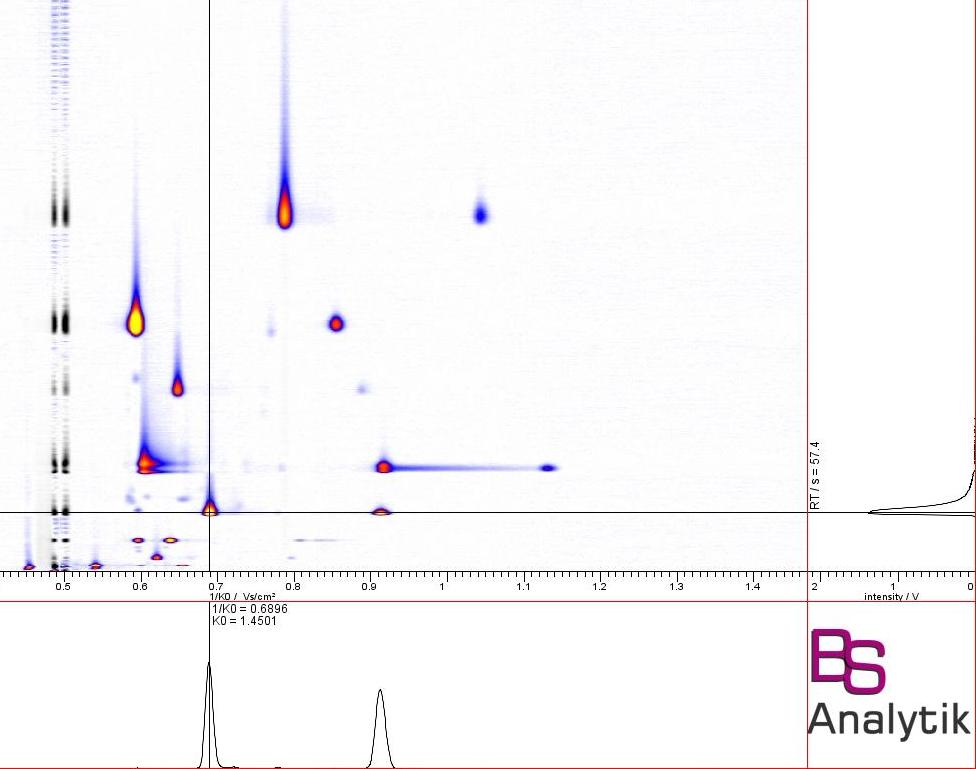
\includegraphics[width = 0.9\textwidth]{bilder/BD15_1304101102_ims}
 \caption{Spektrum einer MCC-IMS-Messung}
 \label{picture:Spektrum1}
\end{figure}
%
Zu beobachten ist, dass schnelle Teilchen Peaks zu frühen Zeitpunkten erzeugen, die eine relativ geringe Varianz aufweisen, hingegen spätere Peaks tendenziell breiter werden. Ideale Peaks haben die Form einer Gaußkurve.


\subsection{Technische Daten}
Eine MCC besteht aus ca. $1000$ Kapillaren mit je
\begin{itemize}
 \item $20\,-\,80$\,\textmu m Durchmesser
 \item Stationäre Phase ist Flüssigkeitsfilm, ca. $0,1\,-\,0,8$\,\textmu m dick
\end{itemize}
 
$\rightarrow$ MCC etwa $2\,-6$\,mm dick und $20$\,cm lang
\todo{Technische Daten belegen}

\begin{figure}
 \centering
  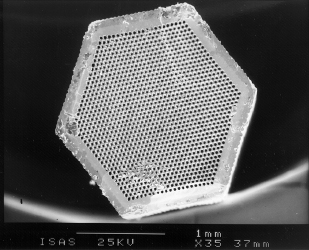
\includegraphics[width = 0.5\textwidth]{bilder/MultiCapillaryColumn}\\
  \caption[Querschnitt einer MCC]{Querschnitt einer MCC \protect\footnotemark}
\end{figure}
\footnotetext{http://yas.yanaco.co.jp/products/import-gc-ims.html}

\subsection{Peakcharakteristika}
Um später die simulierten Peaks mit denen aus den Referenzdatensätzen gut vergleichen zu können, sollen nun einige Eigenschaften aufgeführt werden, die einen Peak beschreiben.

Die offentsichtlichste Eigenschaft ist die Lage des Peaks, genauer gesagt, die Lage des Maximums des Peaks.

Außerdem können die Peaks verschiedene Formen haben. Im theoretischen Idealfall haben sie die Form einer Gaußkurve, jedoch tritt oft ein Tailing auf, welches verschiedene Ursachen haben kann. Unter Anderen seien hier genannt: zusätzliche Adsorptionseffekte, die beim Altern einer Säule auftreten \cite{kolb2003}, technische Ursachen wie kleinste Hohlräume zwischen der Säule und dem Gaseinlass bzw. -Austritt, sowie einige Stoffe, die generell zu Tailing neigen \todo{Zitat, dass einige Stoffe gererell tailen}. 
Beim Tailing steigt die Kurve zunächst stark an, sinkt jedoch nach Erreichen des Maximalwerts deutlich langsamer ab, es entsteht ein Schwanz (engl. Tail). Auch der umgekehrte Fall, Fronting genannt, kann auftreten, ist jedoch in den vorliegenden Datensätzen nicht zu beobachten.

Als drittes können Peaks unterschiedlich breit sein. Da jedoch ein Peak mit größerer Intensität, also möglicherweise größerer Stoffmenge, automatisch auch einen breiteren Peak erzeugt, betrachten wir die Halbwertsbreite als Maß für die Peakbreite. Die Halbwertsbreite wird auf halber Maximalhöhe des Peaks gemessen. Im Fall von auftretendem Tailing oder Fronting ist es sinnvoll, je einen Wert für rechts und links des Maximalwerts zu berechnen.


\section{Probabilistische Arithmetische Automaten}
Ein Probabilistischer Arithmetischer Automat (PAA) nach \cite{MHKR} ist ein Modell, mit dem eine Folge zufälliger Operationen beschrieben werden kann. 
Für PAA existieren Algorithmen, welche eine gemeinsame Verteilung von Zuständen und Werten oder auch die Verteilung der Wartezeit für einen Wert berechnen. Wie in Kapitel \ref{chapter:mod} beschrieben wird, kann das Modell zur Simulation einer Multikapillarsäule auch als PAA formuliert werden. Mit dieser Formulierung ist die Zeit, die zum Durchlaufen einer Säule gebraucht wird, dann die Wartezeit für den Wert, welcher der Länge der Säule entspricht. Deshalb kann ein PAA nützlich sein, um neben der eigentlichen Simulation auch noch eine erwartete Verteilung der Ankunftszeiten der Teilchen zu berechnen. 

Zunächst sei hier eine Definition für den PAA gegeben, anschließend wird der Algorithmus zur Berechnung der Wartezeit beschrieben.
%In diesem Fall ist die Länge der Säule der Wert, auf den gewartet wird und man ist interessiert in der Verteilung der Anzahl der Zeitschritte, die benötigt werden, um die Länge zu erreichen. 

%TODO: Wo soll das rein? Sinnvoll, wenn das zu Beginn erklärt
% Was tut ein PAA

\subsection{Definition eines PAA}
% Formale Definition

\begin{definition}[PAA]
 Ein Probabilistischer Arithmetischer Automat (PAA) ist ein Tupel
 $ \mathcal{P} = (\mathcal{Q}, q_0, T, \mathcal{V}, v_0, \mathcal{E}, (e_q)_{q\in\mathcal{Q}}, (\theta_q)_{q\in\mathcal{Q}})$, dabei ist:
 \begin{itemize}
  \item $\mathcal{Q}$ eine endliche Menge von Zuständen
  \item $q_0 \in \mathcal{Q}$ der Startzustand
  \item $T: \mathcal{Q} \times \mathcal{Q} \rightarrow [0,1]$ eine Übergangsfunktion mit $\sum_{q' \in \mathcal{Q}} T(q, q') = 1 $ das heißt $(T(q,q'))_{q,q' \in \mathcal{Q}}$ ist eine stochastische Matrix
  \item $\mathcal{E}$ eine endliche Menge von Emissionen
  \item $e_q: \mathcal{E} \rightarrow [0,1]$ eine Wahrscheinlichkeitsverteilung der Emissionen für jeden Zustand
  \item $\mathcal{V}$ eine Menge von Werten
  \item $v_0$ der Startwert
  \item $\theta_q: \mathcal{V} \times \mathcal{E} \rightarrow \mathcal{V}$ eine Operation für jeden Zustand
 \end{itemize}
\end{definition}
Dabei entspricht $ \mathcal{P} = (\mathcal{Q}, q_0, T)$ einer Markovkette und $ \mathcal{P} = (\mathcal{Q}, q_0, T, \mathcal{E}, (e_q)_{q\in\mathcal{Q}})$ einem Hidden Markov Model. \todo{Muss ich dann Markov erklären?}

\subsection{Algorithmus zur Berechnung der Wartezeit}

\todo{Algos für die Verteilung und Wartezeit-Berechnung vorstellen}
\chapter{Modell} %Modell/Modelle?
\label{chapter:mod}
%\todo{Kapitelstruktur?}
Im Folgenden werden die Simulationsmodelle für die Chromatographie vorgestellt. 
Zunächst müssen einige Vorgaben festgelegt werden, wie reale Bedingungen in der Simulation abgebildet werden sollen.

Basis für die anschließend vorgestellten Modelle ist der im letzten Kapitel beschriebene Phasenwechsel der Teilchen im Verlauf der Chromatographie. Nach einem sehr einfachen Modell, das mit lediglich zwei Parametern auskommt, wird ein weiteres, komplexeres Modell beschrieben.

Zusätzlich zur Simulation vieler einzelner Teilchen, welche die Modelle durchlaufen, wird auch jeweils eine Modellierung als PAA vorgestellt.

\section{Vorgaben}
Bei jeder Simulation müssen Einschränkungen gegenüber den realen Bedingungen gemacht werden. In diesem Fall betrifft das vor allem drei Punkte: den Raum, die Zeit und die Anzahl der Analytteilchen.

%\section{Festlegung der Einheiten}
Für die Simulation wird eine Multikapillarsäule von $20$ cm Länge angenommen. Diese wird in $1000$ Einheiten von je $0,2$\, mm unterteilt. Damit nutzt die Simulation ein diskretes Raummodell. Außerdem wird nicht berücksichtigt, dass die Säule eine Röhre und damit dreidimensional ist, sondern wird als gerade Strecke angenommen. An jeder der $1000$ Positionen der Strecke können sich jedoch beliebig viele Teilchen aufhalten, ohne aufeinander Einfluss zu nehmen.

Die Zeit wird ebenfalls als diskret und endlich angenommen. Es wird von einem Trägergas ausgegangen, welches nach etwa $0,1$ Sekunden die Säule durchlaufen hat. Außerdem soll es sich pro Zeitschritt und damit pro Simulationsschritt je einen Raumschritt fortbewegen, was einer Geschwindigkeit von $2$ m/s entspricht. Damit entspricht eine Zeiteinheit $0,1/1000$ Sekunden also $0,1$\, ms. Um die Simulationsdauer zu beschränken und da auch reale Experimente nach einer bestimmten Zeit beendet sind, wird eine maximale Zeit von $240$ Sekunden, also $2.400.000$ Simulationsschritten gesetzt. Insbesondere diese Grenze lässt sich aber nach Belieben verändern.

Die gemachten Vorgaben sind in Tabelle \ref{einheiten} zusammengefasst.

\begin{table}[H]
\centering
\caption[Entsprechung der Einheiten]{Festsetzung der Entsprechung der Einheiten zwischen realem Experiment und Simulation}
\label{einheiten}
\begin{tabular}{|l||l|l|}
\hline
			  & MCC                 			& Simulation              \\ \hline \hline
Länge der Säule           & $20$ cm               		& $1000$ Raumschritte       \\ \hline
			  & \multicolumn{2}{l|}{1 Raumschritt $\equiv 0,2$ mm} \\ \hline
Durchlaufzeit Trägergas   & $0,1$ s $\equiv$ $2$ m/s       	& $1000$ Zeitschritte       \\ \hline
			  & \multicolumn{2}{l|}{1 Zeitschritt $\equiv 0,1$ ms} \\ \hline
Geschwindigkeit Trägergas & $2$ m/s 				& 1 Raumschritt / Zeitschritt \\ \hline
\end{tabular}
\end{table}
%\todo{einheiten tabelle}

Die Anzahl der Analytteilchen pro Stoff im Laborexperiment ist viel zu groß, als dass tatsächlich jedes einzelne simuliert werden könnte und dabei in akzeptabler Zeit Ergebnisse erzielt würden. Daher wurde die Anzahl der Teilchen auf $1000$ bzw. $10.000$ beschränkt. Wie sich in den simulierten Daten zeigt, ergeben sich bereits bei $1000$ Teilchen erkennbare Peaks, die jedoch noch von Simulationsdurchlauf zu Simulationsdurchlauf Unterschiede aufweisen können. Bei $10.000$ simulierten Teilchen ergeben sich demgegenüber geglättete Peaks, die sich zwischen den Simulationen nur noch minimal unterscheiden.
%Die Intensität eines Peaks in echten Messungen ist unter anderem abhängig vom Messverfahren und der Stoffmenge im zu analysierenden Gemisch. In den Simulationen wird stets eine bestimmte Anzahl von Teilchen, zum Beispiel $1000$ oder $10000$ Teilchen simuliert.


\section{2-Zustände Modell}
\label{chapter:mod:2p}

Als Grundlage für die Entwicklung eines Simulationsmodells dient die Beobachtung des chromatographischen Prozesses. Dieser ist, wie in Kapitel \ref{chapter:gru} beschrieben, gekennzeichnet durch viele Teilchen, welche häufig zwischen der stationären und mobilen Phase wechseln. Es liegt also nahe, dass im Modell ebenfalls Teilchen simuliert werden, die zwischen zwei Zuständen, welche die beiden Phasen repräsentieren, wechseln. Im Folgenden bezeichnet m die mobile und s die stationäre Phase. Der Phasenwechsel geschieht jeweils mit einer bestimmten Wahrscheinlichkeit. Dabei kann es möglich sein, dass die Wahrscheinlichkeiten für den Wechsel in die eine oder andere Richtung voneinander abhängig sind. Beispielsweise könnte eine hohe Wahrscheinlichkeit in den stationären Zustand zu wechseln, eine ebenfalls hohe Wahrscheinlichkeit, wieder mobil zu werden, bedingen. Da ein solcher Zusammenhang jedoch nicht gegeben sein muss, wird für das Modell zunächst der Fall von unabhängigen Wechselwahrscheinlichkeiten angenommen. Es sei also $p_{\text {m}}$ die Wahrscheinlichkeit, dass ein Teilchen, welches sich bereits in der mobilen Phase befindet, auch mobil bleibt und $1-p_{\text {m}}$ die Wahrscheinlichkeit, dass es in die stationäre Phase übergeht. Analog seien $p_{\text {s}}$ und $1-p_{\text {s}}$ die Wahrscheinlichkeiten, dass ein stationäres Teilchen in der stationären Phase bleibt bzw. zur mobilen Phase wechselt. 

\subsection{Teilchensimulation}
Durch die eben gemachten Annahmen ergibt sich als erstes Modell ein einfacher Automat mit zwei Zuständen $\mathcal{Q} = \{\text{m, s}\}$. m ist Startzustand, da die Teilchen stets nur in der mobilen Phase in die Säule eintreten können. Dazu kommen die oben beschriebenen Transitionen $T= 
\begin{pmatrix}
p_{\text {m}} & 1-p_{\text {m}} \\
1-p_{\text {s}} & p_{\text {s}} 
\end{pmatrix}
$ 
Eine graphische Darstellung des Modells zeigt Abbildung \ref{tikz:2p_Mod} %\todo{Formale Beschreibung meines Modells}

\begin{figure}[ht]
 \centering

\usetikzlibrary{arrows,%
                topaths}%
\tikzstyle{knoten}=[draw,-,thick,fill=none,inner sep=0pt, minimum width=35pt, circle]
\tikzstyle{kante}=[draw,-,thick,black]
\usetikzlibrary{arrows,decorations.pathmorphing,backgrounds,positioning,fit}

\begin{tikzpicture}[->,>=stealth',shorten >=1pt,auto,node distance=5cm,
  thick,main node/.style={circle,draw,font=\sffamily\large\bfseries,text width = 1cm}]

  \node[main node] (s)  {\,\,\,\,\,s};
  \node[main node, minimum width=1.5cm] (m2) [left of=s] {};
  \node[main node] (m) [left of=s] {\,\,\,\,m};

  \path[every node/.style={font=\sffamily}]

    (s)   edge [bend left] node [below] {$1-p_{\text {s}}$} (m2)
            edge [loop right] node {$p_{\text {s}}$} (s)
        
    (m2)  edge [bend left] node [above]{$1-p_{\text {m}}$} (s)
             edge [loop left] node {$p_{\text {m}}$} (m2)
        ;
\end{tikzpicture}
\caption{Graphische Darstellung des 2-Zustände Modells}
\label{tikz:2p_Mod}
\end{figure}

Für die Simulation müssen viele Teilchen, ausgehend vom mobilen Zustand, den Automaten durchlaufen. Dabei wird zusätzlich zum Zustand der Teilchen auch der Ort, an dem sie sich befinden, verwaltet. Wenn sich ein Teilchen im mobilen Zustand befindet, wird dieser Ortszähler erhöht. Die Simulation eines Teilchens ist beendet, wenn der Ortszähler den gewünschten Wert, der der Länge der Trennsäule entspricht, erreicht hat.
Außerdem werden die dafür benötigten Schritte gezählt, woraus sich dann die Ankunftszeit des Teilchens am Ende der Säule ableitet.
Diese Simulation muss für sehr viele Teilchen wiederholt werden, sodass alle Ankunftszeiten zusammen als ein Peak dargestellt werden können.

%leiten sich dann die Ankunftszeiten der Teilchen bei Erreichen eines bestimmten Wertes des Ortszählers ab.

% für abbruchbedingung und zeit für peak
% Das ganze 1000 mal wiederholen da je nur eine kapillare simuliert wurde
In Kapitel \ref{chapter:meth} werden verschiedene Arten der Simulation und jeweils der genaue Ablauf beschrieben.
%Der genaue Ablauf der Simulation wird in Kapitel \ref{chapter:meth} beschrieben.

% Grundlage: Phasenwechsel
% Das eigentliche Modell
% Simulation je einer Kapillare und eines Stoffes -> Viele Durchläufe

\subsection{PAA für das 2-Zustände Modell}
% Modell als PAA
Wie in Kapitel \ref{chapter:gru} erwähnt, kann der chromatographische Prozess auch als PAA modelliert werden. Die nötigen Zustände sind offensichtlich $\mathcal{Q} = \{\text{s, m}\}$ und auch hier ist der Startzustand der mobile Zustand. Auch die Transitionen entsprechen denen im oben beschriebenen Modell. Um den Aufenthaltsort der Teilchen zu modellieren, werden die Werte genutzt. Dementsprechend liegen mögliche Werte im Bereich $\mathcal{V} = \{0, \ldots, \ell\}$ mit dem Startwert $v_0 = 0$. Mit Hilfe der Emissionen wird die Fortbewegung der Teilchen modelliert: Im mobilen Zustand sollen die Analyte um einen Schritt fortbewegt werden, im stationären Zustand nicht. Damit ergeben sich zwei mögliche Emissionen: $\mathcal{E} = \{0, 1\}$. Emission $0$ wird stets und ausschließlich in Zustand s emittiert, gleiches gilt für Emission $1$ und Zustand m. Offensichtlich muss die Emission jeweils auf den Wert addiert werden, daher entspricht $\theta$ der Addition.

Dadurch ergibt sich folgende Definition für den PAA für das 2-Zustände Modell:
\begin{itemize}
 \item $ \mathcal{Q} = \{\text{s, m}\} $
 \item $ q_0 = \text{m}$
 \item $ T = \begin{pmatrix}
	  p_{\text{m}} & 1-p_{\text{m}}  \\
	  1-p_{\text{s}} & p_{\text{s}} \\
	\end{pmatrix} $
 \item $\mathcal{E} = \{0, 1\}$
 \item $ e_{\text{s}}(z)= [\![ z=0 ]\!]$
 \item $ e_{\text{m}}(z) = [\![ z=1 ]\!]$ %\begin{cases}
                  %  1, & \text{wenn } z = 1, \\
                  %  0, & \text{sonst.}
                  % \end{cases}$ %e_{\text{s}}(0) = 1, e_{\text{s}}(1)=0, e_{\text{m}}(0) = 0, e_{\text{m}}(1)=1, 
 \item $   \mathcal{V} = \{0, \ldots, \ell\}$
 \item $ v_0 = 0 $
 \item $ \theta_{\text{s}} = \theta_{\text{m}} = + $
\end{itemize}
 
 %Dabei ist $[\![ b ]\!]$ definiert als $1$ falls die Bedingung $b$ wahr ist und $0$ sonst.
Dabei ist $[\![ b ]\!]$ definiert als 
$\begin{cases}
 1, & \text{wenn } b \text{ wahr ist}, \\
 0, & \text{sonst.}
\end{cases}$

% \todo{iverson bracket definieren}
 
\begin{figure}
 \centering
  \begin{tikzpicture}[->,>=stealth',shorten >=1pt,auto,node distance=3.5cm, thick,
   state node/.style={circle,fill=white,draw,font=\sffamily\bfseries, minimum height=30pt, text width = 1.6cm, align = center},
   operation node/.style= {regular polygon, regular polygon sides=3,  fill = white, draw, inner sep=  0pt},
   emission node/.style={rectangle, fill = lightgray!50, draw, text width = 2cm}]

       % \draw[fill=green] (current page.north west) rectangle (current page.south east);
%  
   \node[state node, minimum width = 2.1cm] (m2) at (2,1) {};
   \node[state node] (m) at (2, 1)  {m};
   \node[state node] (s) [right = of m] {s};
   \node[operation node, align = center] (os)  at (1.5,0.2) {$+$};
   \node[operation node, align = center] (om)  at (8,0.2) {$+$};

   \path[every node/.style={font=\sffamily\large}]

    (s)   edge [bend right] node [above] {$1-p_{\text {s}}$} (m2)
            edge [loop right] node {$p_{\text {s}}$} (s)
        
    (m2)  edge [bend right] node[below]{$1-p_{\text {m}}$} (s)
             edge [loop left] node {$p_{\text {m}}$} (m2)
        ;

   \fill[color=gray!40] (1.1, 4) --(2,1.5) -- (2.9,4) -- cycle ;
   \fill[color=gray!40] (6.55, 4) -- (7.45,1.5) -- (8.35,4) -- cycle ;

   \node[emission node, align = center] (em) [above of = m] {$e_{\text {m}}(0) = 0$\\$e_{\text {m}}(1)=1$};
   \node[emission node, align = center] (es) [above of = s] {$e_{\text {s}}(0) = 1$\\$e_{\text {s}}(1)=0$};
  
  \end{tikzpicture}
  \caption{PAA für das 2-Zustände Modell} \label{PAA_2P}
\end{figure}

Im Abbildung \ref{PAA_2P} ist der PAA für das 2-Zustände Modell graphisch dargestellt.
%TODO: Noch etwas Text, der sich auf \ref{PAA_2P} bezieht

\subsection{Grenzen des Modells}
Eine genaue Analyse der Peaks, die mit dem 2-Zustände Modell erzeugt werden können, findet sich in Kapitel \ref{chapter:eva}. An dieser Stelle sei nur vorweg genommen, dass es zwei Hauptprobleme mit dem Modell zu geben scheint. 

Das erste mögliche Problem ist, dass die Peaks eine Minimalbreite an einem gegebenen Zeitpunkt $t$ haben. Das heißt, dass mit dem Modell keine Peaks simuliert werden können, die ihrem Maximalzeitpunkt an $t$ haben, jedoch schmaler sind als Breite $b$. Ob dieser Umstand ein Problem darstellt, muss anhand realer Messdaten herausgefunden werden.

Das andere Problem ist, dass fast keine der simulierten Peaks ein Tailing aufweisen. Lediglich ein sehr stark eingeschränkter Parameterbereich erzeugt ein Tailing. Leider sind die Maximalzeitpunkte der so erzeugten Peaks alle sehr klein, sodass nicht über die gesamte simulierte Zeit Peaks mit Tailing erzeugbar sind. Darüber hinaus ist Tailing in echten Messungen eher bei späten Peaks zu beobachten.

Um dieses Problem zu lösen, wird im Folgenden ein erweitertes Modell mit drei Zuständen eingeführt, welches es ermöglicht, tailende Peaks zu erzeugen.


\section{3-Zustände Modell} 
\label{chapter:mod:3s}

%TODO Der letzte Absatz zu weiteren möglichen Erweiterungen kann dann als kleiner absatz ganz ans ende des modellkapitels und wird im ausblick noch mal aufgegriffen

Bisher fand keine Unterscheidung zwischen Adsorption und Lösung der Teilchen an bzw. in der stationären Phase statt, sodass zwei Zustände und Transitionen zwischen diesen beiden Zuständen als Modell ausreichten. In der Realität können beide Wechselwirkungen parallel zueinander statt finden: Wenn ein Teilchen in den stationären Zustand wechselt, wird jeweils entschieden, ob es adsorbiert wird oder sich löst.

Außerdem ist es realistisch anzunehmen, dass sich die Wahrscheinlichkeiten, in einen der beiden Zustände überzugehen oder in die mobile Phase zurückzukehren, unterscheiden. Die Wahrscheinlichkeit, dass ein Teilchen adsorbiert wird, kann viel höher oder niedriger sein als die, dass es zur Lösung übergeht. Umgekehrt kann ein Teilchen viel leichter oder schwerer aus der Adsorption in die mobile Phase zurückkehren, als dies beim gelösten Zustand der Fall ist. Daher liegt es nahe, einen neuen Zustand einzuführen, sodass die Adsorption und die Lösung voneinander getrennt behandelt werden. Die Tatsache, dass Tailing, wie bereits anfangs erwähnt, unter anderem durch zusätzliche Adsorptionseffekte verursacht sein kann, lässt vermuten, dass durch diesen dritten Zustand ein Tailing in der Simulation verursacht werden kann. 
 
\begin{figure}[h]
\begin{subfigure}[t]{\textwidth}
\centering
\begin{tikzpicture}[->,>=stealth',shorten >=1pt,auto,node distance=3cm,
  thick,main node/.style={circle,fill=white!20,draw,font=\sffamily\large\bfseries, minimum width = 25pt},
   knoten/.style={thick,fill=none,inner sep=0pt, minimum width=25pt, circle}]
{
  \node[main node] (m) at (0, 0) {m};
  \node[main node] (s1) at (5, 1.5) {a}; 
  \node[main node] (s2) at (5, -1.5) {l};

  \path[every node/.style={font=\sffamily}]
        
    (m)  edge [bend left] node[above left]{$p_{\text{ma}}$} (s1) 
            edge [bend right] node[below left]{$p_{\text{ml}}$} (s2)
             edge [loop left] node {$p_{\text{mm}}$} (m)

    (s2)   edge node [right] {$p_{\text{lm}}$} (m)
            edge [loop right] node {$p_{\text{ll}}$} (s1)
        
    (s1)  edge node [right] {$p_{\text{am}}$} (m)
	  edge [loop right] node {$p_{\text{aa}}$} (s1)

        ;}
\end{tikzpicture}
\hfill
\caption{Getrennte Zustände}
\label{tikz:4p_Mod_a}
\end{subfigure}

\begin{subfigure}[t]{\textwidth}
\centering
\begin{tikzpicture}[->,>=stealth',shorten >=1pt,auto,node distance=3cm,
  thick,main node/.style={circle,fill=white!20,draw,font=\sffamily\large\bfseries, minimum width = 25pt}]
{
   \node[main node] (m) at (0,0) {m}; 
  \node[main node] (s1) at (4,0) {a};
  \node[main node] (s2) at (8,0) {l};

  \path[every node/.style={font=\sffamily}]

    (s2)   edge [bend left] node [below] {$p_{\text{la}}$} (s1)
            edge [loop right] node {$p_{\text{ll}}$} (s1)
        
    (s1)   edge [bend left] node [above] {$p_{\text{al}}$} (s2)
            edge [bend left] node[below] {$p_{\text{am}}$} (m)
			edge [loop above] node {$p_{\text{aa}}$} (s1)
        
    (m)  edge [bend left] node[above]{$p_{\text{ma}}$} (s1)
             edge [loop left] node {$p_{\text{mm}}$} (m)
        ;}
\end{tikzpicture}

\caption{Zwischenzustand}
\label{tikz:4p_Mod_b}
\end{subfigure}
\caption{Mögliche Modelle mit drei Zuständen}
\label{tikz:4p_Mod}
\end{figure}
 
In Abbildung \ref{tikz:4p_Mod} sind zwei Möglichkeiten gezeigt, dem bisherigen Modell einen neuen Zustand hinzuzufügen.
Neben dem mobilen Zustand (m) gibt es in beiden Fällen je zwei stationäre Zustände, einen für die Adsorption (a) und einen für die Lösung (l). Die Übergangswahrscheinlichkeiten zwischen dem alten Zustand $i$ und dem neuen Zustand $j$ sind jeweils $p_{ij}$. 

In Abbildung \ref{tikz:4p_Mod_a} sind die beiden stationären Zustände getrennt voneinander, dazwischen finden keine direkten Übergänge statt. 
Anschaulich kann man sich vorstellen, dass bei Übertritt in die stationäre Phase schon festgelegt wird, welcher Art der Übergang sein wird. Es scheint intuitiv sinnvoll zu sein, die Übergangswahrscheinlichkeiten zu den beiden Zuständen sowie die beiden Wahrscheinlichkeiten, wieder in die mobile Phase einzutreten, sehr unterschiedlich zu wählen. Damit wird bezweckt, dass sie sich nicht einfach wieder zu einer Gesamtwahrscheinlichkeit aufaddieren, die man auch mit dem 2-Zustände Modell hätte erreichen können. In einen der beiden Zustände sollen die Teilchen also nur seltener kommen, dafür aber dort sehr lange verweilen, in den anderen Zustand wechseln die Teilchen häufiger, bleiben aber auch nicht so lange. Außerdem spiegelt dies die in Kapitel \ref{chapter:gru} erwähnte Tatsache wieder, dass adsorbierte Teilchen sich leichter wieder in die mobile Phase begeben können, als dies bei gelösten Teilchen der Fall ist.

In Abbildung \ref{tikz:4p_Mod_b} dient der erste stationäre Zustand als Übergangszustand zum zweiten stationären Zustand. Dabei ist der Übergangszustand die Adsorption als Hinweis darauf, dass die Teilchen, die sich in der stationären Phase lösen, zunächst mit deren Oberfläche in Kontakt treten und zumindest kurzzeitig adsorbiert sind, gleiches gilt für die andere Richtung. Nachdem ein Teilchen adsorbiert wurde, besteht die Möglichkeit, dass es sich noch in der stationären Phase löst oder auch adsorbiert bleibt. Auch hier liegt es nahe, die Wahrscheinlichkeiten für die verschiedenen Übergänge so zu gestalten, dass die Teilchen in einem der stationären Zustände seltener aber länger bleiben.

Beide Fälle können zu einem Gesamtmodell mit drei Zuständen zusammengefasst werden. Das Modell hat die Zustände $\mathcal{Q} = \{\text{m, a, l}\}$. m ist wie auch im 2-Zustände Modell der Startzustand. Aus den oben angegebenen Übergangswahrscheinlichkeiten ergibt sich dann die Transitionsmatrix 
\begin{equation}
T= 
\begin{pmatrix}
p_{\text{mm}} &  p_{\text{ma}} & p_{\text{ml}} \\
p_{\text{am}} &  p_{\text{aa}} & p_{\text{al}} \\
p_{\text{lm}} &  p_{\text{la}} & p_{\text{ll}} 
\end{pmatrix}
\label{3s_Transit}
\end{equation}
  
In Modell 3a sind die Wahrscheinlichkeiten für $p_{\text{al}}$ und $p_{\text{la}}$ immer $0$ und in 3b gilt dies entsprechend für $p_{\text{ml}}$ und $p_{\text{lm}}$.

In den späteren Abschnitten der Arbeit ist mit dem 3-Zustände Modell oft das Modell 3a gemeint, da sich in ersten Auswertungen der beiden Modelle ergeben hat, dass sich damit tailende Peaks erzeugen lassen, für das Modell 3b wurden bei diesen oberflächlichen Untersuchungen keine solche Peaks gefunden. Die später vorgestellten Methoden und deren Implementierungen können aber alle Varianten des 3-Zustände Modells simulieren.

Die Parameter, die für das Modell 3a betrachtet werden, sind \pmm, \pml, \paa\ und \pll, die übrigen drei Parameter lassen sich aus diesen berechnen.


\subsection{PAA}
Analog zum PAA für nur zwei Zustände kann für drei Zustände ein PAA definiert werden. Aus Gründen der Übersicht wird hier nur das Gesamtmodell mit drei Zuständen und allen dazwischen möglichen Übergängen berücksichtigt. Für die Modelle 3a und 3b müssen auch für den PAA nur die entsprechenden Wahrscheinlichkeiten angepasst werden.

\begin{figure}
 \begin{tikzpicture}[->,>=stealth',shorten >=1pt,auto,node distance=3cm, thick,
  state node/.style={circle,fill=white,draw,font=\sffamily\bfseries, minimum height=30pt, text width = 1.5cm, align = center},
  operation node/.style= {regular polygon, regular polygon sides=3,  fill = white, draw, inner sep=  0pt},
  emission node/.style={rectangle, fill = lightgray!50, draw, text width = 2cm}]
 
  \node[state node] (m) at (2, 0) {m};
  \node[state node] (s1) at (8, 2) {a}; 
  \node[state node] (s2) at (8, -2) {l};

  \node[operation node, align = center] (om)  at (1.5,-0.8) {$+$};
  \node[operation node, align = center] (os1)  at (8.5, 1.5) {$+$};
  \node[operation node, align = center] (os2)  at (8.5,-2.5) {$+$};

  \path[every node/.style={font=\sffamily\large}]

    (m) edge [loop left] node {$p_{\text{mm}}$} (m)
			edge [bend left] node [above] {$p_{\text{ma}}$} (s1)
            edge [bend left = 10] node [below]{$p_{\text{ml}}$} (s2)
        
    (s1)  edge [bend left = 10] node[above]{$p_{\text{am}}$} (m) 
             edge [loop above] node {$p_{\text{aa}}$} (s1)
 			edge [bend left] node[right]{$p_{\text{al}}$} (s2)
    
    (s2)  edge [bend left] node[below]{$p_{\text{lm}}$} (m)
 			 edge [bend left] node[right]{$p_{\text{la}}$} (s1)	
             edge [loop below] node {$p_{\text{ll}}$} (s2)
        ;

   \fill[color=lightgray!40] (1.1, 2.5) --(2,0.9) -- (2.9,2.5) -- cycle ;
   \fill[color=lightgray!40] (8.9, 2) -- (10,1.5) -- (10,2.5) -- cycle ;
   \fill[color=lightgray!40] (8.9, -2) -- (10,-1.5) -- (10, -2.5) -- cycle ;
% 
   \node[emission node, align = center] (em) [right of= s1] {$e_{\text{a}}(0) = 1$\\$e_{\text{a}}(1)=0$};
   \node[emission node, align = center] (em) [right of = s2] {$e_{\text{l}}(0) = 1$\\$e_{\text{l}}(1)=0$};
   \node[emission node, align = center] (es) [above of = m] {$e_{\text{m}}(0) = 0$\\$e_{\text{m}}(1)=1$};
  
\end{tikzpicture}

\caption{PAA für das allgemeine 3-Zustände Modell}
\label{3sPAA}
\end{figure}

Eine graphische Darstellung des PAA für drei Zustände ist in Abbildung \ref{3sPAA} gegeben. Der stationäre Zustand wurde in zwei Zustände aufgeteilt, sodass $\mathcal{Q} = \{\text{m, a, l}\}$. m bleibt Startzustand. Die Transitionen wurden entsprechend der Transitionsmatrix \ref{3s_Transit} angepasst. An den Werten ändert sich im Vergleich zum PAA für 2-Zustände nichts, da weiterhin die gleiche Säulenlänge $\ell$ zu erreichen ist. Ebenso bleibt die Addition für alle Zustände $z$ als Operation $\theta_z$ bestehen. Bezüglich der Emissionen ändert sich am mobilen Zustand nichts und die beiden stationären Zustände übernehmen das gleiche Verhalten des bisherigen stationären Zustandes, da sich in beiden die Analyte nicht fortbewegen.
Der PAA für das 3-Zustände Modell ist also definiert als:

\begin{itemize}
 \item $ \mathcal{Q} = \{\text{m, a, l}\}  $
 \item $  q_0 = \text{m} $
 \item $ T = \begin{pmatrix}
  p_{\text{mm}} & p_{\text{ma}} & p_{\text{ml}} \\
  p_{\text{am}} & p_{\text{aa}} & p_{\text{ll}} \\
  p_{\text{lm}} & p_{\text{la}} & p_{\text{ml}} \\
 \end{pmatrix} $
 \item $  \mathcal{E} = \{0, 1\} $
 \item $ e_{\text{m}}(z) = [\![ z=1 ]\!]$
 \item $  e_{\text{a}}(z) = e_{\text{l}}(z) = [\![ z=0 ]\!]$
 \item $  %e_{\text{m}}(1) = e_{\text{a}}(0) = e_{\text{l}}(0) = 1, e_{\text{m}}(0) = e_{\text{a}}(1) = e_{\text{l}}(1) = 0,
 \mathcal{V} = \{0, \ldots, \ell\} $
 \item $ v_0 = 0 $
 \item $  \theta_{\text{m}} = \theta_{\text{a}} = \theta_{\text{l}} = + $
\end{itemize}

\section{Weitere Modelle}

Eine weitere Möglichkeit, das Modell zu verändern, besteht darin, das Gleichgewicht, welches sich zwischen den beiden Phasen aufbaut, zu berücksichtigen. Damit müssten die Wahrscheinlichkeiten, den Zustand zu wechseln, nicht mehr fest vorgegeben sein, sondern sich dynamisch während der Simulation aus der aktuellen Verteilung der Teilchen an einem bestimmten Ort auf die Zustände berechnen. Das würde dazu führen, dass Teilchen, die sich zu Beginn des Pulks befinden, mit einer höheren Wahrscheinlichkeit in die stationäre Phase oder eine der stationären Phasen übergehen, Teilchen in der Mitte haben demgegenüber eine deutlich geringere Wahrscheinlichkeit, stationär zu werden, da nun das Gleichgewicht gehalten werden muss. Die Veränderung der Übergangswahrscheinlichkeiten hinge demnach auch von der Quote der Teilchen ab, die dann schon wieder mobil geworden sind. Teilchen am Ende des Pulks sollten demnach nur sehr selten noch in eine stationäre Phase wechseln können. Genau diese Teilchen würden jedoch einen Tail verursachen, da sie sich, nach dem Übergang in die mobile Phase, hinter dem Pulk befinden würden.

Eine sehr ähnliche Idee ist es, noch eine Sättigung der freien Plätze zur Adsorption einzubauen. Unabhängig vom Gleichgewicht zwischen den Phasen, kann es möglich sein, dass sehr viele Teilchen bereits mit der Oberfläche interagieren. Weitere Teilchen, die sich an den Rand der Säule begeben haben dann möglicherweise kaum noch Kontaktmöglichkeiten mit der stationären Phase, sodass sich ihre Wahrscheinlichkeit, mobil zu bleiben, erhöht.

% Erweiterung um weiteren (stat) Zustand um Unterschied zwischen Lösung und Adsorption zu haben
% Ideen zur Geschwindigkeit und warum das Quatsch ist. ?
\chapter{Methoden} 
\label{chapter:meth}

In diesem Kapitel werden für die verschiedenen Modelle Möglichkeiten beschrieben, diese zu simulieren. Offensichtlich ist es möglich, tatsächlich jeden einzelnen Zeitschritt für alle Teilchen zu betrachten. Wenn Zustandswechsel jedoch nicht sehr häufig vorkommen, kann es viel Zeit einsparen, nur zu relevanten Zeitpunkten, also für jeden Zustandswechsel, zu simulieren und dabei den Zeitpunkt des nächsten Wechsels zu notieren.

Im zweiten Abschitt des Kapitels wird beschieben, wie der PAA umgesetzt werden kann. Dabei liegt der Fokus auf einer eingeschränkten Variante des PAA, bei dem einige nicht benötigte Funktionalitäten, wie beispielsweise je Zustand verschiedene Operationen oder mehrere mögliche Emissionen, nicht berücksichtigt werden.


\section{Simulation}
Zunächst betrachten wir das in \ref{chapter:mod:2p} vorgestellte Modell mit nur zwei Zuständen und zwei Parametern, anschließend auch die in \ref{chapter:mod:3s} beschriebene Erweiterung auf 3 Zustände und damit bis zu 6 Parameter.

Die Ankunftszeiten der simulierten Teilchen können dann als Peak aufgefasst und dargestellt werden. Außerdem werden daraus die resultierenden Peakdaten berechnet.
%Nach erfolgter Simulation können aus den Ankunftszeiten der Teilchen die Peakdaten der resultierenden Peaks berechnet werden.

\todo{Berechnung der Peakdaten, wohin}

\subsection{Simulation des 2-Parameter Modells}
Für das 2-Parameter Modell wurden zwei verschiedene Möglichkeiten der Simulation entworfen. Die erste, ``Step-by-Step'', simuliert schrittweise alle Zeitpunkte eines Säulendurchlaufs. Die zweite, ``By-Event'' verwaltet eine Liste relevanter Zeitpunkte, an denen Ereignisse - im konkreten Fall: Zustandswechsel - statt finden.

\subsubsection{Step-by-Step}
\begin{algorithm}
\caption{Ablauf der Step-by-Step Simulation}
\label{algo_by_Step}
\begin{algorithmic}
\REQUIRE Zustandsliste $s= [s_1 = 1, \ldots, s_n=1]$, Ortsliste $o=[o_1=0, \ldots , o_n=0]$, Zeit $t=0$, Maximalzeit $t_{max}$
\ENSURE Ankuftszeiten $r$
\WHILE{$t < t_{max}$ \AND $len(s) > 0$}
\FORALL {$p$}
\STATE Simuliere $p$
\IF {$o_p >l$}
\STATE $r \leftarrow t$
\STATE Lösche $s_p$ und $o_p$
\ENDIF
\ENDFOR
\STATE $t +=1$
\ENDWHILE
\RETURN $r$
\end{algorithmic}
\end{algorithm}

\todo{Hinweis auf Parallelisierbarkeit und andere Zeitverbesserungen hier oder in Implementierung}

%TODO: Zustand $s \in \{0, 1\}$ Ort $o \in \{0, \ldots, l\}$ wobei $l$ die Länge der Säule ist. -> in text einbauen


Der Ablauf einer Simulation ist in Algorithmus \ref{algo_by_Step} gegeben.

Für jedes Teilchen $p$ muss jeweils der aktuelle Zustand $s$ und Ort $o$ festgehalten werden, außerdem muss der aktuelle Zeitpunkt $t$ vermerkt werden. Da nur zwei Zustände existieren, bietet es sich an, dafür ein Array mit booleschen Werten zu verwenden. $0$ steht dabei für stationär und $1$ für mobil. Die Identifikation der Teilchen geschieht dabei über ihre Postition im Array.
\todo{Array oder Vektor, bzw ohne Parallelisierbarkeit, da ja eigentlich nicht nötig?}
%Für jedes Teilchen wird in einem zweiten Array an gleicher Position sein aktueller Ort gespeichert. 

Die Teilchen wechseln in jedem Schritt mit einer bestimmten Wahrscheinlichkeit den Zustand. Diese sei $pm$ für das Verweilen in der mobilen Phase, $ps$ für das Verweilen in der stationären Phase und $1-pm$ bzw. $1-ps$ für die beiden Möglichkeiten des Phasenwechsels. Daher muss pro Schritt und Teilchen eine Zufallszahl gezogen werden, anhand derer sich entscheidet, wie es sich verhält. Außerdem muss in jedem Schritt der Ort für jedes mobile Teilchen um eins erhöht werden.

Zum Ablauf der Simulation wurde entschieden, dass zunächst die Entscheidung über die Phase gefällt wird und sich anschließend die Teilchen gemäß ihres neuen Zustandes bewegen. Außerdem starten alle Teilchen ganz zu Beginn in der mobilen Phase, da sie nur so in das System eintreten können.

\begin{figure}
\begin{tikzpicture}[->,>=stealth',shorten >=1pt,auto,node distance=4cm,
  thick,main node/.style={circle,fill=white!20,draw,font=\sffamily\large\fseries}]
\tikzstyle{feld}=[draw,minimum width=1.5cm,minimum height=0.7cm,font=\sffamily\footnotesize]


\begin{scope}[start chain =1 going right, node distance =0.0mm]
	\node [on chain =1, feld, draw=none] {Phasen};
	\node [on chain=1, feld, fill=blue!30!white] (p1) {0};
	\node [on chain=1, feld] (p3) {0};
	\node [on chain=1, feld, fill=green!30!white] (p4) {1};
	\node [on chain=1, feld] (p5) {1};
	\node [on chain=1, feld,fill=magenta!70!blue!20!white] (p6) {1};
	\node [on chain=1, feld] (p7) {1};
	\node [on chain=1, feld, fill=orange!30!white] (p8) {0};
\end{scope}

\begin{scope}[start chain =1 going right, node distance =0.0mm,shift={(0cm, -1cm)}]
	\node [on chain =1, feld, draw=none] {Orte};
	\node [on chain=1, feld] (o1) {0};
	\node [on chain=1, feld] (o3) {4};
	\node [on chain=1, feld] (o4) {4};
	\node [on chain=1, feld] (o5) {1};
	\node [on chain=1, feld] (o6) {6};
	\node [on chain=1, feld] (o7) {6};
	\node [on chain=1, feld] (o8) {3};
\end{scope}

\begin{scope}[start chain =1 going right, node distance =0.0mm,shift={(0cm, -2.5cm)}]
	\node [on chain =1, feld, draw=none] {ZV};
	\node [on chain=1, feld] (z1) {$0,9$};
	\node [on chain=1, feld] (z3) {$0,6$};
	\node [on chain=1, feld] (z4) {$0,2$};
	\node [on chain=1, feld] (z5) {$0,9$};
	\node [on chain=1, feld] (z6) {$0,7$};
	\node [on chain=1, feld] (z7) {$0,2$};
	\node [on chain=1, feld] (z8) {$0,3$};
\end{scope}

\begin{scope}[start chain =1 going right, node distance =0.0mm,shift={(0cm, -3.5cm)}]
	\node [on chain =1, feld, draw=none] {$p_s = 0,8$};
	\node [on chain=1, feld, fill=blue!30!white] (ps1) {0};
	\node [on chain=1, feld] (ps3) {1};
	\node [on chain=1, feld] (ps4) {1};
	\node [on chain=1, feld] (ps5) {0};
	\node [on chain=1, feld] (ps6) {1};
	\node [on chain=1, feld] (ps7) {1};
	\node [on chain=1, feld, fill=orange!30!white] (ps8) {1};
\end{scope}

\begin{scope}[start chain =1 going right, node distance =0.0mm,shift={(0cm, -4.5cm)}]
	\node [on chain =1, feld, draw=none] {$p_m = 0,5$};
	\node [on chain=1, feld] (pm1) {0};
	\node [on chain=1, feld] (pm3) {0};
	\node [on chain=1, feld, fill=green!30!white] (pm4) {1};
	\node [on chain=1, feld] (pm5) {0};
	\node [on chain=1, feld,fill=magenta!70!blue!20!white] (pm6) {0};
	\node [on chain=1, feld] (pm7) {1};
	\node [on chain=1, feld] (pm8) {1};
\end{scope}

\begin{scope}[start chain =1 going right, node distance =0.0mm, shift={(0cm, -6cm)}]
	\node [on chain =1, feld, draw=none] {Phasen};
	\node [on chain=1, feld, fill=blue!30!white] (np1) {1};
	\node [on chain=1, feld] (np3) {0};
	\node [on chain=1, feld, fill=green!30!white] (np4) {1};
	\node [on chain=1, feld] (np5) {0};
	\node [on chain=1, feld,fill=magenta!70!blue!20!white] (np6) {0};
	\node [on chain=1, feld] (np7) {1};
	\node [on chain=1, feld, fill=orange!30!white] (np8) {0};
\end{scope}

\begin{scope}[start chain =1 going right, node distance =0.0mm,shift={(0cm, -7cm)}]
	\node [on chain =1, feld, draw=none] {Orte};
	\node [on chain=1, feld] (no1) {1};
	\node [on chain=1, feld] (no3) {4};
	\node [on chain=1, feld] (no4) {5};
	\node [on chain=1, feld] (no5) {1};
	\node [on chain=1, feld] (no6) {6};
	\node [on chain=1, feld] (no7) {7};
	\node [on chain=1, feld] (no8) {3};
\end{scope}

\end{tikzpicture}
\caption{Prinzip der schrittweisen Simulation bei zwei Parametern}
\label{2p_by_step}
\end{figure}

In Abbildung \ref{2p_by_step} ist eine schematische Darstellung eines Simulationsschritts zu finden. Hier werden die Teilchen alle parallel bearbeitet 
\todo{müsste hier nicht schon ein verweis auf numpy hin?}
Um eine Abfrage des aktuellen Zustand zu sparen, wird einfach für beide Möglichkeiten berechnet. \todo{benennung der pspmvektoren}
Dadurch können alle Zustandswechsel ebenfalls parallel über die Formel: $(p \land pm) \lor (\lnot p \land \lnot ps)$ berechnet werden.
Für die neuen Orte kann einfach der neue Zustandsvektor auf den alten Ortsvektor addiert werden.

Nach jedem solchen Simulationsschritt wird getestet, ob Teilchen bereits den Wert von $l$ erreicht und damit die ganze Säule durchlaufen haben. Die entsprechende Anzahl dafür benötigter Schritte entspricht der Ankunftszeit der Teilchen und wird festgehalten, sodass als Ergebnis am Ende der Simulation eine Liste von Ankunftszeiten aller Teilchen entsteht. Teilchen, die angekommen sind, werden aus beiden Vektoren gelöscht.

Die Simulation ist beendet, wenn alle Teilchen das Säulenende erreicht haben, also die Vektoren eine Länge von $0$ haben. 
Als alternative Abbruchbedingung kann eine maximale Anzahl von Simulationsschritten gewählt werden, nach deren Ablauf die Simulation beendet ist, wenn nur Peaks von Interesse sind, die vor diesem Zeitpunkt im Chromatogramm erscheinen.

\todo{Wo stehen Zeiteinheiten festgelegt -> ImAnplementierung}


\subsubsection{By-Event}

\todo{Beide Algo: Invalidflag?}
\begin{algorithm}
\caption{Ablauf der by-Event Simulation}
\label{algo_by_event}
\begin{algorithmic}
\REQUIRE Eventliste $e= [e_0 = [(s_0, o_0), \ldots, (s_n, o_n)]]$ mit $s_p = 1, o_p = 0$, $\forall p$ , Zeit $t=0$, Maximalzeit $t_{max}$
\ENSURE Ankuftszeiten $r$
\WHILE{$t<t_{max}$ \AND Länge $e> 0$}
%\STATE Teilchenliste $= e[t]$
\FORALL {$(s_p, o_p)$ in $e[t]$}
\IF {$o_p > l$}
\STATE Berechne $t_a(p)$ 
\STATE $r \leftarrow t_a(p)$
\STATE Lösche $(s_p, o_p)$
\ELSE
\STATE Simuliere $(s_p, o_p)$
\STATE Aktualisiere $e$
\ENDIF
\ENDFOR
\STATE $t+=1$
\ENDWHILE
\RETURN $r$
\end{algorithmic}
\end{algorithm}

Der Ablauf der ereignisbasierten Simulation ist in \ref{algo_by_event} angegeben.

Dabei muss für jeden Zeitpunkt $t$ verwaltet werden, welche Teilchen zu diesem Zeitpunkt ihren Zustand wechseln. Jedes Teilchen besteht dabei aus seinem Ort und seinem Zustand. 
Zunächst starten alle Teilchen wie bei der schrittweisen Simulation bei Zeitpunkt $1$, Ort $0$ und mobil.
Ein Simulationsschritt behandelt dann alle Teilchen eines Zeitpunktes. Ein solches Event beinhaltet den Wechsel des Zustands, die Bestimmung des Zeitpunkts des nächsten Zustandswechsels sowie bei mobilen Teilchen eine Änderung des Ortes. Anschließend wird das Teilchen der Zeitpunkteliste seines nächsten Aktionszeitpunktes hinzugefügt. Sind alle Teilchen abgearbeitet, wird der Zeitpunkt gelöscht und der nächste Zeitpunkt, an dem etwas passieren soll, bearbeitet.

\begin{figure}
\begin{subfigure}[t]{\textwidth}
\begin{tikzpicture}[->,>=stealth',shorten >=1pt,auto,node distance=4cm,
  thick,main node/.style={circle,fill=white!20,draw,font=\sffamily\large\bfseries}]
\tikzstyle{feld}=[draw,minimum width=1.5cm,minimum height=0.7cm,font=\sffamily\footnotesize]

\begin{scope}[start chain =1 going right, node distance =-0.3mm]
	\node [on chain =1, feld, draw=none,minimum width=2cm] {Events $e$};
	\node [on chain=1, feld,minimum width=2cm] (p2) {$e_2$};
	\node [on chain=1, feld,minimum width=2cm] (p3) {$e_3$};
	\node [on chain=1, feld,minimum width=2cm] (p5) {$e_5$};
	\node [on chain=1, feld,minimum width=2cm] (p7) {$e_7$};
	\node [on chain=1, feld,minimum width=2cm] (p12) {$e_{12}$};
\end{scope}

\begin{scope}[start chain = 1 going below,shift={(2cm, -2cm)}, node distance=0.5cm]
	\node[on chain = 1, feld, fill=green!50!white] (1x1) {($s_1, o_1$)};
	\node[on chain = 1, feld, fill=blue!40!white] (1x2) {($s_4, o_4$)};
	\node[on chain = 1, feld, fill=orange!50!white] (1x3) {($s_7, o_7$)};
\end{scope}

\begin{scope}[start chain = 1 going below,shift={(4cm, -2cm)}, node distance=0.5cm]
	\node[on chain = 1, feld] (2x1) {($s_0, o_0$)};
	\node[on chain = 1, feld] (2x2) {($s_8, o_8$)};
\end{scope}

\begin{scope}[start chain = 1 going below,shift={(6cm, -2cm)}, node distance=0.5cm]
	\node[on chain = 1, feld] (3x1) {($s_{10}, o_{10}$)};
\end{scope}

\begin{scope}[start chain = 1 going below,shift={(8cm, -2cm)}, node distance=0.5cm]
	\node[on chain = 1, feld] (4x1) {($s_2, o_2$)};
	\node[on chain = 1, feld] (4x2) {($s_3, o_3$)};
	\node[on chain = 1, feld] (4x3) {($s_9, o_9$)};
\end{scope}

\begin{scope}[start chain = 1 going below,shift={(10cm, -2cm)}, node distance=0.5cm]
	\node[on chain = 1, feld] (5x1) {($s_5, o_5$)};
\end{scope}

\path [line width=1.4pt, line cap=rect, draw](p2) edge (1x1) ;
\path [line width=1.4pt, line cap=rect, draw](1x1) edge (1x2) ;
\path [line width=1.4pt, line cap=rect, draw](1x2) edge (1x3) ;

\path [line width=1.4pt, line cap=rect, draw](p3) edge (2x1) ;
\path [line width=1.4pt, line cap=rect, draw](2x1) edge (2x2) ;

\path [line width=1.4pt, line cap=rect, draw](p5) edge (3x1) ;

\path [line width=1.4pt, line cap=rect, draw](p7) edge (4x1) ;
\path [line width=1.4pt, line cap=rect, draw](4x1) edge (4x2) ;
\path [line width=1.4pt, line cap=rect, draw](4x2) edge (4x3) ;

\path [line width=1.4pt, line cap=rect, draw](p12) edge (5x1) ;

\end{tikzpicture}
\label{2p_by_event_a}
\caption{Vor der Simulation des Events $e_1$}
\vspace*{5mm}
\end{subfigure}
\begin{subfigure}[b]{\textwidth}
\begin{tikzpicture}[->,>=stealth',shorten >=1pt,auto,node distance=4cm,
  thick,main node/.style={circle,fill=white!20,draw,font=\sffamily\large\bfseries}]
\tikzstyle{feld}=[draw,minimum width=1.5cm,minimum height=0.7cm,font=\sffamily\footnotesize]

\begin{scope}[start chain =1 going right, node distance =-0.3mm]
	\node [on chain =1, feld, draw=none,minimum width=2cm] {Events $e$};
	\node [on chain=1, feld,minimum width=2cm] (p2) {$e_2$};
	\node [on chain=1, feld,minimum width=2cm] (p5) {$e_5$};
	\node [on chain=1, feld,minimum width=2cm] (p7) {$e_7$};
	\node [on chain=1, feld,minimum width=2cm] (p9) {$e_9$};
	\node [on chain=1, feld,minimum width=2cm] (p12) {$e_{12}$};
	\node [on chain=1, feld,minimum width=2cm] (p16) {$e_{16}$};
\end{scope}


\begin{scope}[start chain = 1 going below,shift={(2cm, -2cm)}, node distance=0.5cm]
	\node[on chain = 1, feld] (2x1) {($s_0, o_0$)};
	\node[on chain = 1, feld] (2x2) {($s_8, o_8$)};
\end{scope}

\begin{scope}[start chain = 1 going below,shift={(4cm, -2cm)}, node distance=0.5cm]
	\node[on chain = 1, feld] (5x1) {($s_{10}, o_{10}$)};
	\node[on chain = 1, feld, fill=green!50!white] (5x2) {($s_1, o_1$)};
\end{scope}

\begin{scope}[start chain = 1 going below,shift={(6cm, -2cm)}, node distance=0.5cm]
	\node[on chain = 1, feld] (7x1) {($s_2, o_2$)};
	\node[on chain = 1, feld] (7x2) {($s_3, o_3$)};
	\node[on chain = 1, feld] (7x3) {($s_9, o_9$)};
\end{scope}

\begin{scope}[start chain = 1 going below,shift={(8cm, -2cm)}, node distance=0.5cm]
	\node[on chain = 1, feld, fill=orange!50!white] (9x1) {($s_7, o_7$)};
\end{scope}

\begin{scope}[start chain = 1 going below,shift={(10cm, -2cm)}, node distance=0.5cm]
	\node[on chain = 1, feld] (12x1) {($s_5, o_5$)};
\end{scope}

\begin{scope}[start chain = 1 going below,shift={(12cm, -2cm)}, node distance=0.5cm]
	\node[on chain = 1, feld, fill=blue!40!white] (16x1) {($s_4, o_4$)};
\end{scope}

%\path [line width=1.4pt, line cap=rect, draw](1x2) edge (1x3) ;

\path [line width=1.4pt, line cap=rect, draw](p2) edge (2x1) ;
\path [line width=1.4pt, line cap=rect, draw](2x1) edge (2x2) ;

\path [line width=1.4pt, line cap=rect, draw](p5) edge (5x1) ;
\path [line width=1.4pt, line cap=rect, draw](5x1) edge (5x2) ;

\path [line width=1.4pt, line cap=rect, draw](p7) edge (7x1) ;
\path [line width=1.4pt, line cap=rect, draw](7x1) edge (7x2) ;
\path [line width=1.4pt, line cap=rect, draw](7x2) edge (7x3) ;

\path [line width=1.4pt, line cap=rect, draw](p9) edge (9x1) ;

\path [line width=1.4pt, line cap=rect, draw](p12) edge (12x1) ;

\path [line width=1.4pt, line cap=rect, draw](p16) edge (16x1) ;

\end{tikzpicture}

\label{2p_by_event_b}
\caption{Nach der Simulation}
\end{subfigure}

\caption{Prinzip der ergeignisbasierten Simulation bei zwei Parametern} 
\end{figure}
Wann ein Teilchen das nächste Mal seinen Zustand wechselt, wird mit Hilfe einer geometrisch verteilten Zufallszahl bestimmt. Daher lohnt sich diese Art der Simulation insbesondere bei Parametern nahe 1. 
Wenn ein Teilchen im aktuellen Schritt in den mobilen Zustand gewechsel hat, muss auch sein Ort angepasst werden. Da sich Teilchen eine Raumeinheit pro Zeitschritt bewegen, wird der Ort entsprechend der Zufallszahl erhöht.
TODO: Ort

Allerdings gestaltet sich das Testen auf Erreichen der Säulenlänge bei dieser Methode etwas schwieriger, da $l$ nur sehr selten genau getroffen wird. In vielen Fällen wird ein Teilchen von einem Ort kleiner $l$ direkt auf einen viel größeren Ort befördert. Daher muss zwischen jedem Simulationsschritt getestet werden, ob ein Teilchen bereits $l$ überschritten hat. Wenn das der Fall ist, muss mit Hilfe der Differenz zum aktuellen Simulationszeitpunkt die korrekte Ankunftszeit des Teilchens berechet werden.
Ob diese Berechnung nach jedem Simulationsschritt, also vor Neueintragung in die Liste geschieht, oder vor jedem Schritt, ist egal. Allerdings muss im zweiten Fall beachtet werden, dass, falls als Abbruchbedingung eine Maximalzeit gewählt wurde, sichergestellt sein muss, dass alle übrigen Teilchen noch einmal auf Erreichen von $l$ getestet werden.



\subsection{Simulation des 3-Zustände Modells}

Analog zum 2-Parameter Modell kann auch das 3-Zustände Modell schrittweise oder ereignisbasiert umgesetzt werden. Die Algorithmen \ref{algo_by_Step} und \ref{algo_by_event} bleiben jeweils unverändert, lediglich die Umsetzung der Simulation eines Schrittes bzw. einer Ereignisliste muss angepasst werden.

\subsubsection{Step-by-Step}
Weiterhin die neue Zustandsberechnung als logische Verknüpfung
Um aus Zufallszahlen die passenden Arrays mit größer/kleiner-Abfrage zu machen, erstelle kumulierte Wahrscheinlichkeiten (ein mal zu beginn)
Viele Hilfsarrays nötig, die entsprechend viel überflüssige Information enthalten
Erweiterung auf mehr Zustände mit exakt diesem Vorgehen wohl kaum sinnvoll, da zu zeitaufwändig. (TODO: Diskussionskapitel?)

\subsubsection{By-Event}
Bei dieser Simulationsart sind nur minimale Anpassungen notwendig. Es wird ein weiterer Zustand eingeführt und die Wahrscheinlichkeiten angepasst.
Da pro Schritt immer Zustandswechsel hier hilfsmatrix mit angepassten übergangswahrscheinlichkeiten, bei der die Wechselwahrscheinlichkeiten normiert 
werden


\section{PAA}

Zur Nutzung des PAA könnte man einfach die bereits vorhandene mosdi-Implementierung nutzen. Da diese jedoch mit steigender Säulenlänge deutlich langsamer wird \todo{Laufzeitverweis mosdi} wurde eine neue Herangehensweise gewählt. Diese zeichnet sich vor allem dadurch aus, dass einige nicht benötigte Funktionalitäten eines PAA nicht umgesetzt werden. 
Dies betrifft die Möglichkeit je Zustand mehrere verschiedene Emissionen mit einer jeweiligen Wahrsscheinlichkeit zuzulassen. Es wird, wie in \ref{PAA_2P} und TODO paa3s zu sehen ist, nur jeweils eine Wert mit der Wahrscheinlichkeit $1$ emittiert. Außerdem wird keine Möglichkeit weitere Operationen zuzulassen benötigt, Addition genügt. Da darüber hinaus nur im mobilen Zustand überhaupt eine Veränderung des Wertes erfolgt, wird der PAA auf diese Möglichkeit beschränkt.
Außerdem wird nicht jeweils die vollständige Zustands-Werte-Verteilung betrachtet, sondern nur der tatsächlich relevante Bereich. Dieser Bereich umfass zu Beginn einer Simulation lediglich die bereits erreichbaren Werte.
Für alle n<l ist n der maximal erreichbare Wert in schritt n
Außerdem werden Werte sehr nah bei 0 (<10hoch-17) ignoriert. Solche Werte werden aus der Verteilung gelöscht und die dadurch benötigten Arrays verkürzt, wodurch wiederum Simulationszeit eingespart wird.

%todo Wie werden die neuen Einträge berechnet? Graphik, Text dazu

% todo Wie werden die Arrays gekürzt

\subsection{PAA für das 2-Parameter Modell}

Ähnlich wie bei der Simulation der Teilchen 

\begin{figure}

\begin{tikzpicture}[->,>=stealth',shorten >=1pt,auto,node distance=4cm,
  thick,main node/.style={circle,fill=white!20,draw,font=\sffamily\large\bfseries}]
\tikzstyle{feld}=[draw,minimum width=2cm,minimum height=1cm,font=\sffamily\scriptsize]

\begin{scope}[start chain=1 going right,node distance=-0.0mm]
    \node [on chain=1,feld,draw=none, font=\small] {stat.};
    \node [on chain=1,feld] (s1) {$s_1$};
    \node [on chain=1,feld] (s2) {$s_2$};
    \node [on chain=1,feld] {$s_3$};
    \node [on chain=1,feld] {$s_4$};
    \node [on chain=1,feld,draw=none] {$\ldots$};
%     \node [on chain=1,feld,draw=none] {$\ldots$};
%     \node [on chain=1] {\textbf{Text}};
\end{scope}


\begin{scope}[start chain=1 going right,node distance=-0.0mm, shift={(0cm,-1.2cm)},start chain=circle placed {at=(-\tikzchaincount*60:1.5)}]
    \node [on chain=1,feld,draw=none, font=\small] {mob.};
    \node [on chain=1,feld] (m1) {$m_1$};
    \node [on chain=1,feld] (m2) {$m_2$};
    \node [on chain=1,feld] {$m_3$};
    \node [on chain=1,feld] {$m_4$};
    \node [on chain=1,feld,draw=none] {$\ldots$};
%     \node [on chain=1,feld,draw=none] {$\ldots$};
%     \node [on chain=1] {\textbf{Text}};
\end{scope}

\begin{scope}[start chain=1 going right,node distance=-0.0mm, shift={(0cm,-2.6cm)},start chain=circle placed {at=(-\tikzchaincount*60:1.5)}]
    \node [on chain=1,feld,draw=none, font=\small] {s\_to\_s };
    \node [on chain=1,feld] (ss1) {$s_1*p_s$};
    \node [on chain=1,feld] (ss2) {$s_2*p_s$};
    \node [on chain=1,feld] {$s_3*p_s$};
    \node [on chain=1,feld] {$s_4*p_s$};
    \node [on chain=1,feld,align=center] {$0$};
%     \node [on chain=1,feld,draw=none] {$\ldots$};
%     \node [on chain=1] {\textbf{Text}};
\end{scope}
\begin{scope}[start chain=1 going right,node distance=-0.0mm, shift={(0cm,-3.8cm)},start chain=circle placed {at=(-\tikzchaincount*60:1.5)}]
    \node [on chain=1,feld,draw=none, font=\small] {s\_to\_m};
    \node [on chain=1,feld,align=center](sm1) {$0$};
    \node [on chain=1,feld] (sm1) {$s_1(1-p_s)$};
    \node [on chain=1,feld] (sm2) {$s_2(1-p_s)$};
    \node [on chain=1,feld] {$s_3(1-p_s)$};
    \node [on chain=1,feld] {$s_4(1-p_s)$};
%     \node [on chain=1,feld,draw=none] {$\ldots$};
%     \node [on chain=1] {\textbf{Text}};
\end{scope}

\begin{scope}[start chain=1 going right,node distance=-0.0mm, shift={(0cm,-5cm)},start chain=circle placed {at=(-\tikzchaincount*60:1.5)}]
    \node [on chain=1,feld,draw=none, font=\small] {m\_to\_m };
    \node [on chain=1,feld,align=center] {$0$};
    \node [on chain=1,feld] (mm1){$m_1*p_m$};
    \node [on chain=1,feld] (mm2){$m_2*p_m$};
    \node [on chain=1,feld] {$m_3*p_m$};
    \node [on chain=1,feld] {$m_4*p_m$};
%     \node [on chain=1,feld,draw=none] {$\ldots$};
%     \node [on chain=1] {\textbf{Text}};
\end{scope}

\begin{scope}[start chain=1 going right,node distance=-0.0mm, shift={(0cm,-6.2cm)},start chain=circle placed {at=(-\tikzchaincount*60:1.5)}]
    \node [on chain=1,feld,draw=none, font=\small] {m\_to\_s};
    \node [on chain=1,feld](ms1) {$s_1(1-p_s)$};
    \node [on chain=1,feld] (ms2){$s_2(1-p_s)$};
    \node [on chain=1,feld] {$s_3(1-p_s)$};
    \node [on chain=1,feld] {$s_4(1-p_s)$};
    \node [on chain=1,feld,align=center] {$0$};
%     \node [on chain=1,feld,draw=none] {$\ldots$};
%     \node [on chain=1] {\textbf{Text}};
\end{scope}

\begin{scope}[start chain=1 going right,node distance=-0.0mm, shift={(0cm, -7.6cm)}]
    \node [on chain=1,feld,draw=none, font=\small] {stat};
    \node [on chain=1,feld,align=center] (s'1) {$s_1*p_s +$\\$m_1(1-p_m)$};
    \node [on chain=1,feld,align=center](s'2) {$s_2*p_s +$\\$m_2(1-p_m)$};
    \node [on chain=1,feld,align=center] {$s_3*p_s +$\\$m_3(1-p_m)$};
    \node (n2) [on chain=1,feld,align=center] {$s_4*p_s +$\\$m_4(1-p_m)$};
    \node [on chain=1,feld,align=center] {$0$};
    \node [on chain=1,feld,draw=none] {$\ldots$};
%     \node [on chain=1,feld,draw=none] {$\ldots$};
%     \node [on chain=1] {\textbf{Text}};
\end{scope}


\begin{scope}[start chain=1 going right,node distance=-0.0mm, shift={(0cm,-8.8cm)},start chain=circle placed {at=(-\tikzchaincount*60:1.5)}]
    \node (n1) [on chain=1,feld,draw=none, font=\small] {mob};
    \node [on chain=1,feld] {$0$};
    \node [on chain=1,feld,align=center] (m'1){$m_1*p_m$\\$s_1(1-p_s)$};
    \node [on chain=1,feld,align=center] (m'2){$m_2*p_m$\\$s_4(1-p_s)$};
    \node [on chain=1,feld,align=center] {$m_3*p_m$\\$s_4(1-p_s)$};
    \node [on chain=1,feld,align=center] {$m_4*p_m$\\$s_4(1-p_s)$};
    \node [on chain=1,feld,draw=none] {$\ldots$};
%     \node [on chain=1,feld,draw=none] {$\ldots$};
%     \node [on chain=1] {\textbf{Text}};
\end{scope}%         ;

\path [line width=1.4pt, line cap=rect, draw=blue!70!red, bend left=30](s1) edge (ss1) ;
\path [line width=1.4pt, line cap=rect, draw=blue!70!red, bend left=30](ss1) edge (s'1) ;
\path [line width=1.4pt, line cap=rect, draw=blue!50!white, bend right=30](m1) edge (ms1) ;
\path [line width=1.4pt, line cap=rect, draw=blue!50!white, bend right=05](ms1) edge (s'1) ;

\path [line width=1.4pt, line cap=rect, draw=green!70!black, bend left=70](m2) edge (mm2) ;
\path [line width=1.4pt, line cap=rect, draw=green!70!black, bend left=40](mm2) edge (m'2) ;
\path [line width=1.4pt, line cap=rect, draw=green!40!yellow, bend right=10](s2) edge (sm2) ;
\path [line width=1.4pt, line cap=rect, draw=green!40!yellow, bend right=40](sm2) edge (m'2) ;

\end{tikzpicture}


\caption{PAA} \label{paa2p_prinzip}
\end{figure}

In \ref{paa2p_prinzip} ist exemplarisch dargestellt, wie die sich neuen Wahrscheinlichkeitsverteilungen in jedem Schritt berechnen. 
Gegeben sind die alten Wahrscheinlichkeitsverteilungen $stat$ und $mob$.
Um auf die neue Verteilung für den stationären Zustand zu kommen, muss für jede Position berechnet werden, welcher Anteil Teilchen stationär bleibt (s\_to\_s) und welcher Anteil bisher mobiler Teilchen in den stationären Zustand wechselt (m\_to\_s).
Analog müssen für die mobile Verteilung die mobil bleibenden sowie die sich aus dem Zustand lösenden Anteile berechnet werden. Da sich die Teilchen in der mobilen Phase jeweils einen Ort vorwärts bewegen, wird hier zusätzlich der ganze Vektor um ein Feld verschoben. Um eine anschließenden parallelen Berechnung der Wahrscheinlichkeiten der beiden Phasen durchführen zu können, wird zum Ausgleich den neu stationären Teilchenmassen ein neues Feld mit der Wahrscheinlichkeit von $0$ angehängt werden


\subsection{PAA für das 3-Zustände Modell}
Wie bei der schrittweisen Teilchensimulation tritt auch beim PAA für das 3-Zustände Modell das Problem auf, dass nicht mehr nur boolesche Werte  ausreichen, um den Zustand zu beschreiben. 

Erklaerung anschaulich auf dem Zettel vom 10.6.15


\section{Berechnung der Peakdaten}
Sowohl für die Simulation vieler Teilchen als auch bei der Verwendung eines PAA müssen nach der Simulation noch die Peakdaten berechnet werden. 

Bei den Teilchensimulationen liegen die Peaks als Liste von Ankuftszeiten vor, beim PAA hingegen als Anteil der Gesamtwahrscheinlichkeit zu jedem Zeitpunkt. 

Besonders bei den Teilchensimulationen ist es vorteilhaft, jeweils mehrere Zeitpunkte zusammen zu fassen, um die Peaks zu glätten.
\todo{Bild unzusammengefasster Daten zur Verdeutlichung?}

Maximalstelle: Am häufigsten vorkommende Ankunftszeit bzw. argmax der Wahrscheinlichkeiten

Breite und Schiefe: Jeweils Quartile berechnen und daraus IQR und IQK
%implementierung.tex

\chapter{Implementierung}
\label{chapter:imp}
\todo{Kapitel Implementierung schreiben}
\todo{Soll hier auch erwähnt werden, wie die verschiedenen Auswertungen gemacht wurden? Plots etc}

Aufrufe der wichtigen Funktionen (der Simulationen) Kommandozeilenparameter mit angeben. 


\section{Teilchensimulation}
Für die Teilchensimulation wurden die Algorithmen \ref{algo_by_Step} und \ref{algo_by_event} jeweils für zwei und drei Zustände implementiert. Dafür wurde Python 3.4 verwendet. 
Um insbesondere bei der Step-by-Step Implementierung eine schnelle Verarbeitung der Zustands- und Ortsarrays zu gewährleisten, wurden dafür NumPy-Arrays verwendet. Außerdem stellt NumPy Methoden zur Berechnung von Percentilen, geometrisch verteilte Zufallszahlen und Bestimmung der Position des größten Wertes einer Liste zur Verfügung, welche für die Implementierung genutzt wurden.
Für die graphische Ausgabe der Peaks und weitere geplottete Darstellungen im Bereich der Auswertung der Simulationen wurde PyPlot genutzt.

% Zur Simulation der beiden Modelle wurde Python 3.4 verwendet. Dabei existieren Abhängigkeiten von NumPy (Arrays zur schnellen Verarbeitung), SciPy (Berechnung von Peakdaten) und PyPlot (graphische Darstellung)

Die Datei \texttt{simulation.py} enthält alle Funktionen zur Simulation und Berechnung der Peakdaten. Wichtigster Bestandteil ist die abstrakte Klasse \texttt{Simulation} und die zwei Unterklassen \texttt{Simulation\_2s} und \texttt{Simulation\_3s}. Wie im vorherigen Kapitel gesehen, unterscheiden sich sowohl bei der Step-by-Step, als auch bei der By-Event Variante die Algorithmen nur durch die Umsetzung eines Berechnungsschrittes, sodass die Methoden zur Simulation eines Berechnungsschrittes bzw. Events in der Superklasse abstrakt sind und jeweils für das Modell passend in den Unterklassen implementiert wurden. In der Klasse \verb!Simulation_3s! sind zusätzlich auch die Vorberechnungen für die kumulierte Parametermatrix der Step-by-Step Simulation und die Wechselmatrix der By-Event Simulation zu finden.

Um eine Simulation zu starten, wird zunächst eine Instanz der Simulationsklasse erstellt

TODO

In der Datei \texttt{plottings} sind mehrere verschiedene Möglichkeiten zur Auswertungen der Simulation enthalten, die unter Anderem auch verwendet wurden, um die Darstellungen in Kapitel \ref{chapter:eva} zu erstellen. 

Die Dateien \verb!2s_simulate_and_plot.py! sowie  \verb!3s_simulate_and_plot.py! sind für das Starten der Simulationen und Plotten der Ergebnisse durch den Benutzer gedacht. Durch den Aufruf mit einigen Kommandozeilenparametern kann zunächst ein vordefinierte Menge an Parameterkombinationen zur Simulation ausgewählt werden. 
Mit dem Parameter \texttt{-p} wird eine Menge von Parameterkombinationen ausgewählt. Zur Verfügung stehen dabei für das 2-Zustände Modell und das 3-Zustände Modell 3a jeweils \textit{small\_set}, \textit{medium\_set} und \textit{large\_set}, außerdem können mittels \textit{random} zufällige Kombinationen erstellt werden, die Anzahl dieser zufälligen Kombinationen wird über den Parameter \texttt{-cn} festgelegt. Außerdem steht für das 2-Zustände Modell noch die Kombination \textit{skew} zur Verfügung, die tailing erzeugende Parameter enthält.

Der Parameter \texttt{-a} wählt den gewünschten Ansatz, also \texttt{-a=S} für die Step-by-Step Simulation und \texttt{-a=E} für die By-Event Simulation.

Mit den Parametern \texttt{-n} und \texttt{-l} können Anzahl der Teilchen und Länge der Säule eingegeben werden. Als Default-Werte dafür sind $1000$ Teilchen und eine Länge von $1000$ Schritten vorgesehen.

Um einen einzelnen Peak zu Plotten, kann mittels \texttt{-pp} die gewünschte Parameterkombination aus $ps$ und $pm$ eingegeben werden. Für die 2-Zustände Simulation würde beispielsweise der Aufruf \verb!python3 2s_simulate_and_plot.py -pp 0.999 0.5! eine Simulation mit den Parametern $ps = 0.999$ und $pm = 0.5$ erstellen, diese simulieren, falls sie noch nicht vorhanden ist und anschließend eine graphische Darstellung des Peaks ausgeben. 
Für die 3-Zustände Simulation ist das Modell 3a als Voreinstellung gewählt, damit kann eine Parameterkombination aus pmm, pml, paa und pll eingegeben werden. Um das gesamte 3-Zustände Modell auszunutzen, ist die Auswahl \texttt{-m=3s} nötig, und die Eingabe aller neun Parameter. 

Weitere Kommandozeilenparameter erlauben die Auswahl der gewünschten Plots.


Sowohl bei der Umsetzung der Step-by-Step Methode als auch By-Event kann mit der Implementierung des 3-Zustände Modells auch das 2-Zustände Modell simuliert werden, indem nicht benötigte Übergangswahrscheinlichkeiten auf einen Wert von $0$ gesetzt werden. Die 2-Zustände Simulation ist aber vor allem bei der Step-by-Step Implementierung deutlich schneller, da nur auf boolschen Werten gearbeitet werden muss und deutlich weniger ungenutzte Information in den Zwischenschritten berechnet wird.


\subsection{Step-by-step}

Im Laborexperiment wird nur in gewissen Intervallen die Ankunft von Teilchen detektiert, bei der MCC-IMS-Kopplung wird beispielsweise nur zwei Mal pro Sekunde eine Messung durchgeführt. Daher genügt es auch in der Simulation, wenn nicht nach jedem Simulationsschritt die Orte aller Teilchen getestet werden, um ein ausreichend exaktes Ergebnis zu erhalten.
Es können also zunächst viele Simulationsschritte durchgeführt werden, bevor getestet wird, ob Teilchen die Länge $l$ erreicht haben. Nach den oben angegebenen Einheiten können so zwischen jedem Test $50$ Simulationsschritte erfolgen, was $0,5 s$ entspricht. Dadurch entfallen viele Abfragen und es kann Simulationszeit eingespart werden. 

Da außerdem klar ist, dass frühestens nach $l$ Schritten Teilchen überhaupt die Säule durchlaufen haben können, muss vor diesem Zeitpunkt auch kein Test auf Erreichen der Länge durchgeführt werden, wodurch weitere Zeit eingespart werden kann.
\todo{wie viel Zeit ist das jeweils? ist das interssant?}


\subsection{By-Event}
%Bei Übergangswahrscheinlichkeiten, die sehr groß oder klein sind, kommt es selten zu Zustandsänderungen, sodass es in diesem Fall effizienter ist, eine Wartezeitmethode zu nutzen: Es wird für jedes Teilchen entschieden, wann es den Zustand wechselt und, falls es mobil ist, wie weit es bis dahin weiter wandert. Es werden also nur die tatsächlichen Ereignisse simuliert, Schritte für Zeitpunkte, zu denen nichts passiert, entfallen.
%\todo{by event-simulation beschreiben -> Methoden}
???

\subsection{Laufzeitvergleich von Step-by-Step und By-Event}

Die Laufzeit einer Simulation hängt stark von den gewählten Parametern ab, außerdem gibt es gravierende Unterschiede zwischen dem 2- und 3-Zustände Modell.

In Tabelle \ref{2s_laufzeit} ist eine Übersicht über die Laufzeiten der verschiedenen Simulationsarten gegeben. 
Jede Zeile enthält die Zeiten für die gegebenen Parameter, jede Spalte entspricht einer Simulationsart. Dabei steht ``S'' für die schrittweise und ``E'' für die ereignisbasierte Simulation, die Zahl dahinter gibt die Anzahl der simulierten Teilchen an.

Die Zeiten wurden unter jeweils gleichen Bedingungen gemessen und sind in Sekunden angegeben. Mit einem $*$ gekennzeichnete Zeiten deuten an, dass die Simulationen nach Erreichen der maximalen Anzahl Simulationsschritte beendet wurden, also keinen vollständigen Peak innerhalb dieses Zeitraumes liefern.

\begin{table}[h]
\centering
\caption{Laufzeitvergleich für die 2-Zustände Simulation}
\label{2s_laufzeit}
\begin{tabular}{|l|l||l|l|l|l|l|l|l|} \hline
ps     & pm   & S,$1000$ & E,$1000$ & S,$10.000$ & E,$10.000$ & PAA & PAA* & MoSDi \\ \hline \hline
$0,997  $ & $ 0,01 $ & $ 8,4  $ & $ 20,9  $ & $ 47,4  $ & $98,2  $ & $  $ & $ $ & $  $\\ \hline
$0,997  $ & $ 0,3  $ & $ 6,1  $ & $ 15,4  $ & $ 33,7  $ & $69,3  $ & $  $ & $ $ & $  $\\ \hline
$0,997  $ & $ 0,6  $ & $ 3,6  $ & $ 8,9   $  & $ 19,4 $ & $40,1  $ & $  $ & $ $ & $  $\\ \hline
$0,997  $ & $ 0,95 $ & $ 0,6  $ & $ 1,3   $  & $ 2,6  $ & $5,4   $ & $  $ & $ $ & $  $\\ \hline
$0,999  $ & $ 0,01 $ & $ 25,5 $ & $ 40,2  $ & $ 142,7 $ & $124,5 $ & $  $ & $ $ & $  $\\ \hline
$0,999  $ & $ 0,3  $ & $ 18,6 $ & $ 27,8  $ & $ 100,4 $ & $88    $ & $  $ & $ $ & $  $\\ \hline
$0,999  $ & $ 0,6  $ & $ 11,0 $ & $ 16,1  $ & $ 57,8  $ & $51    $ & $  $ & $ $ & $  $\\ \hline
$0,999  $ & $ 0,95 $ & $ 1,7  $ & $ 2,2   $ & $ 7,6   $ & $7,1   $ & $  $ & $ $ & $  $\\ \hline
$0,9993 $ & $ 0,01 $ & $ 37,6 $ & $ 47,6  $ & $ 204,1 $ & $140,4 $ & $  $ & $ $ & $  $\\ \hline
$0,9993 $ & $ 0,3  $ & $ 26,6 $ & $ 32,7  $ & $ 143,4 $ & $99,3  $ & $  $ & $ $ & $  $\\ \hline
$0,9993 $ & $ 0,6  $ & $ 15,3 $ & $ 19,6  $ & $ 82,6  $ & $57,6  $ & $  $ & $ $ & $  $\\ \hline
$0,9993 $ & $ 0,95 $ & $ 2,3  $ & $ 2,5   $ & $ 10,8  $ & $8,1   $ & $  $ & $ $ & $  $\\ \hline
$0,9996 $ & $ 0,01 $ & $ 59,9*$ & $ 54,3* $ & $341,2* $ & $167,8*$ & $  $ & $ $ & $  $\\ \hline
$0,9996 $ & $ 0,3  $ & $ 46,2 $ & $ 39,5  $ & $ 252,6 $ & $125,4 $ & $  $ & $ $ & $  $\\ \hline
$0,9996 $ & $ 0,6  $ & $ 26,7 $ & $ 22,4  $ & $ 150,2 $ & $72,8  $ & $  $ & $ $ & $  $\\ \hline
$0,9996 $ & $ 0,95 $ & $ 4,1  $ & $ 3,0   $ & $ 18,8  $ & $10,2  $ & $  $ & $ $ & $  $\\ \hline
\end{tabular}
\end{table}

Wie zu erwarten war, steigt die Laufzeit an, je größer ps und je kleiner pm ist. Das liegt offensichtlich an der Abbruchbedingung des Algorithmus, der terminiert, wenn alle Teilchen über die gesamte Strecke von $\ell$ Schritten simuliert wurden. Simulationsparameter mit kleinem ps oder großem pm sorgen für weniger Verweilen der Teilchen im stationären Zustand und damit eine schnelle Passage der Strecke, wodurch die die Simulationsdauer kürzer wird. 

Bei der Simulation den 2-Zustände Modells ist die Step-by-Step Variante für die meisten Parameterkombinationen deutlich schneller, als die By-Event Implementierung. Der große Vorteil von Step-by-Step liegt hier in der Verwendung von booleschen Werten und Nutzung von NumPy-Arrays, auf welchen die Ausführung logischer Operationen sehr schnell erfolgen kann. 
Mit größer werdendem pm verringert sich der Unterschied zwischen den beiden Simulationsarten, ab einem sehr großen Wert für $p_{\text{m}}$, ab etwa $0,99$ ist die By-Event Variante geringfügig schneller. Das liegt daran, dass in diesen Fällen besonders selten Ereignisse erzeugt werden müssen und sich die Teilchen in großen Sprüngen forbewegen können. 

\todo{stand bis hier irgendwas davon, dass ich 3a verwende?}
Anders sieht die Situation bei der Simulation des 3-Zustände Modells aus. Tabelle \ref{3s_laufzeit} bietet eine Übersicht über die Laufzeiten mit verschiedenen Parametern.

\begin{table}[h]
\centering
\caption{Laufzeitvergleich für die 3-Zustände Simulation}
\label{3s_laufzeit}
\begin{tabular}{|l|l|l|l||l|l|l|l|l|l|l|}
\hline
pmm & pml & paa & pll & S, $1000$ & E, $1000$ & S, $10.000$ & E, $10.000$ \\ \hline \hline
$ 0,01 $ & $0,00005$ & $0,997$  & $0,99995$  & $26,2   $ & $23,9  $ & $123,7 $ & $ $  \\ \hline
$ 0,01 $ & $0,00005$ & $0,997$  & $0,999995$ & $47,4   $ & $24,4  $ & $150 $ & $ $  \\ \hline
$ 0,01 $ & $0,00005$ & $0,9996$ & $0,99995$  & $170,8* $ & $35,9* $ & $870* $ & $ $  \\ \hline
$ 0,01 $ & $0,00005$ & $0,9996$ & $0,999995$ & $169,7* $ & $35,4* $ & $869* $ & $ $  \\ \hline
$ 0,01 $ & $0,003 $  & $0,997$  & $0,99995$  & $36,2   $ & $25,2  $ & $150,6 $ & $ $  \\ \hline
$ 0,01 $ & $0,003 $  & $0,997$  & $0,999995$ & $118,8**$ & $31,5**$ & $390,7**$ & $ $  \\ \hline
$ 0,01 $ & $0,003 $  & $0,9996$ & $0,99995$  & $170*   $ & $34,8* $ & $870* $ & $ $  \\ \hline
$ 0,01 $ & $0,003 $  & $0,9996$ & $0,999995$ & $170*   $ & $29,9* $ & $871* $ & $ $  \\ \hline
$ 0,9  $ & $0,00005$ & $0,997$  & $0,99995$  & $5      $ & $2,6 $   & $15,5 $ & $ $  \\ \hline
$ 0,9  $ & $0,00005$ & $0,997$  & $0,999995$ & $28,4   $ & $2,7 $   & $44,3 $ & $ $  \\ \hline
$ 0,9  $ & $0,00005$ & $0,9996$ & $0,99995$  & $22,5   $ & $3,9 $   & $98 $ & $ $  \\ \hline
$ 0,9  $ & $0,00005$ & $0,9996$ & $0,999995$ & $49,9   $ & $4 $     & $126,1 $ & $ $  \\ \hline
$ 0,9  $ & $0,003 $  & $0,997$  & $0,99995$  & $16,9   $ & $3,3 $   & $43 $ & $ $  \\ \hline
$ 0,9  $ & $0,003 $  & $0,997$  & $0,999995$ & $108,3**$ & $4,3** $ & $294,2* $ & $ $  \\ \hline
$ 0,9  $ & $0,003 $  & $0,9996$ & $0,99995$  & $30,1   $ & $4,0 $   & $120 $ & $ $  \\ \hline
$ 0,9  $ & $0,003 $  & $0,9996$ & $0,999995$ & $115,6**$ & $4,7** $ & $ $ & $ $  \\ \hline
\end{tabular}
\end{table}
Für die 3-Zustände Simulation müssen in der Step-by-Step Implementierung sehr viele Einträge für die Hilfsarrays erzeugt werden, die jedoch für die Berechnung der neuen Arrays nicht benötigt werden. Durch diese überflüssigen Berechnungen verliert die Step-by-Step Implementierung ihren Vorteil gegen über der By-Event Variante, sodass diese schneller wird. Dies wird noch deutlicher, je größer $p_{\text{mm}}$ wird.

%Bei Parametern nah an $1$ lohnt meist die Nutzung der By-Event Implementierung, da dann nur seltener Ereignisse erzeugt werden und viele Schritte in denen nichts passiert, also kein Zustandswechsel stattfindet, übersprungen werden können.
%Bei sehr vielen Teilchen lohnt sich eher die Step-by-Step Variante, da die Teilchen, die in NumPy-Arrays als boolesche Werte vorliegen, sehr viel schneller verarbeitet werden können, als die Listen, die bei der Event -Variante verwendet werden. Eine weitere Parallelisierung scheint hier aber nicht zu lohnen
%Zumindest bei Parametern extrem nah bei 1 kann sich die Laufzeit der By-Event stark vergrößern, wenn die Säule zu kurz ist, da die Teilchen ``viel zu weit über das Ziel hinausschiessen'', aber das erst später festgestellt wird, wenn das Teilchen wieder betrachtet wird und schon entsprechend viele Zeitschritte vergangen sind. 

% Generelles: Welche Sprachen, warum (?)
% Die Simulation in Python, beide Varianten (Also by-event und step-by-step) 
% -> Algorithmen?

\section{Simulation des PAA}
Die Berechnung des PAA existiert in Java, dabei Referenz auf mosdi (Zitiere Paper, in dem das vorgestellt wird und sage, dass ich das verwende)

In der Hoffnung, Laufzeit einzusparen durch eine eingeschränkte Version des PAA und Nutzung von Julia, wurde eine eigene Implementierung entwickelt.

%(laufzeit linear/quadratisch oder so in irgendwas? noch mal bei mosdi nachgucken) länge sowieso beschränkt durch länge der säule (?????) und nicht durch maximale wartezeit

Warum Julia? 

Laufzeitvergleich bei gleichen Ergebnissen

Die Nachbearbeitung der Ergebnisse des PAA wurde wiederum in Python implementiert.



%evaluation.tex

\chapter{Evaluation}
\label{chapter:eva}
\todo{Kapitel Evaluation schreiben}

Was kann ich mit meinem Modell?

Simulation von Peaks die ideal-gaußförmig sind oder tailing aufweisen

Grenzen des Modells:
Minimalbreite kann nicht unterschritten werden


Formel zur Umrechnung von Peakdaten in Parameter, oder falls das nicht drin ist, zumindest Zusammenhänge, dazu zb Plots von drei festen Parametern
Evtl Tabelle mit exemplarischen Daten?
Sinnvolle Parameterbereiche

3a modell liefert tailing, welches bei 3b nicht gefunden wurde (vielleicht einfach nur die falschen parameter ausprobiert?)

\section{Relevanter Parameterbereich / relevate Peaks}

\todo{Strukur: erst komplett 2p dann 3s, wegen referenz auf schiefe bei 2p in den params für 3s}

\subsection{2-Parameter Modell}


\subsection{3-Zustände Modell}
\todo{Wo erwähnen, dass nach 240 sec Schluss ist?}


Die wenigen Peaks, die beim 2-Parameter Modell Schiefe aufweisen dienen als Grundlage für eine sinnvolle Parametereinschränkung für pml und pll. Dabei war zu beobachten, dass die Teilchen nur selten in den stationären Zustand eintreten, dafür aber sehr lange dort verweilen. Um diesen Effekt nachzuahmen, muss pml dementsprechend sehr klein im Vergleich zu pma und pmm sein. pll muss dafür sehr groß sein, deutlich größer als paa

In der experimentellen Phase der Arbeit wurden zunächst im gesamten Parameterraum $[0;1]^3$ einige Simulationen durchgeführt, um herauszufinden, in welchen Bereichen sich Peaks ergeben. 
Durch die Beschränkung des Spektrums auf $240$ Sekunden scheiden schon viele Parameterkombinationen aus, welche spätere Peaks erzeugen würden. Das betrifft insbesondere diejenigen Kombinationen, die eine geringe Wahrscheinlichkeit haben, mobil zu bleiben oder zu werden, dafür aber mit einer sehr hohen Wahrscheinlichkeit stationär werden oder bleiben. 
% Für die Schiefe soll es zunächst keine Beschränkungen geben, TODO (gibt es ne sinnvolle Obergrenze, Optik mit Werten vergleichen)
Typischerweise sind Peaks zu Beginn des Spektrums eher schmal, spätere Peaks können breiter werden. Generell lässt sich sagen, dass der IQR eines Peaks geringer sein sollte, als sein Maximalzeitpunkt. Darüber hinaus wurde eine maximale Peakbreite von 10+0.2*maxzeitpunkt TODO festgelegt. Peaks mit höherem IQR sind in einem Spektrum kaum noch als Peaks zu erkennen.
Sehr breite Peaks sind auch nur dann als Peak zu erkennen, wenn sie sehr schief sind.
Für die Schiefe gilt, dass ein Tailing ab einem IQK von 0.2 gut zu erkennen ist. Werte bis 0.4 treten meist bei schiefen Peaks auf, die auch optisch einem realistischen Peak ähneln. Darüber hinaus haben die Peaks oft ein sehr langes Tailing, welches teilweise auch über die Maximalzeit hinausragt. Dieses ist jedoch auf einem so niedrigen Niveau, dass es in einem Spektrum mit Rauschen wahrscheinlich unter gehen würde.
\todo{bewertende aussagen weglassen, habe ja keine vergleichsdaten}
Dadurch ergeben sich folgende Einschränkungen für die verschiedenen Parameter:
\begin{itemize}
 \item $p_{mm}$: keine generellen Einschränkungen, es wurden für Werte im Intervall $[0,005; 0,99]$ Peaks gefunden. Bei noch kleineren Werten TODO bei größeren Werten TODO
 \item $p_{ml}$: sinnvolle Werte liegen im Bereich $[0,00001; 0,001]$. Bei kleineren Werten ergeben sich auch Peaks, die jedoch kein oder fast kein Tailing mehr aufweisen, sodass auch auf das zwei-Parameter-Modell zurückgegriffen werden kann. Bei größeren Werten verweilen die Teilchen so lange im gelösten Zustand, dass die Peaks extrem breit werden, insbesondere, wenn der Parameter $p_{ll}$ auch sehr groß gewählt wurde.
 \item $p_{aa}$: für diesen Parameter wurde der das Intervall auf $[0.997, 0.9996]$ beschränkt. Kleinere Werte sorgen für extrem frühe Peaks. Diese könnten zwar berücksichtigt werden, unterscheiden sich jedoch kaum voneinander. Bei größeren Werten werden die Peaks meist zu breit und zu spät. 
 \item $p_{ll}$: sinnvolle Werte liegen im Bereich $[0,9999; 0,999995]$. Kleinere Werte TODO Bei größeren Werten werden die Teilchen so lange im stationären Zustand gehalten, dass die Peaks meist über das Maximum von 240 Sekunden hinausragen oder zu breit werden. Dies gilt insbesondere, wenn für $p_{ml}$ ebenfalls ein großer Wert gewählt wurde. Im oberen Bereich des Intervalls (>0.999995 erzeugen werden hier Peaks erzeugt, die eine sehr große Schiefe aufweisen, wo der Tail jedoch (wahrscheinlich) im Rauschen verschwindet. Mit den aktuellen Maßen lässt sich das kaum zeigen, wird jedoch beim Blick auf einen geplotteten Peak sofort klar.
\end{itemize}

In allen Fällen gilt jedoch, dass auch jeweils die Kombination der Parameter berücksichtigt werden muss, insbesondere, wenn ein Parameter am Rand des jeweils angegebenen Intervalls liegt, kommt es häufig vor, dass er nur in einigen wenigen Kombinationen für realistische Peaks sorgt.
Beispiele: TODO: ein paar Kombis nennen, die grenzwertig, bzw drüber hinaus sind.



\section{Einfluss der verschiedenen Parameter auf Peaks}

\subsection{2-Parameter Modell} 

Sowohl Zeitpunkt als auch Breite der Peaks hängen von ps und pm ab.
Nur in einem sehr kleinen Bereich, bei dem die Peaks ihren Maximalzeitpunkt bei etwa TODO haben, tritt überhaupt Schiefe auf. 


\subsection{3-Zustände Modell}

In den meisten Fällen kann ein deutlicher Zusammenhang zwischen den Parametern und Peakdaten beobachtet werden, diese seien im Folgenden aufgeführt.
Für den Maximalzeitpunkt des Peaks sowie seine Breite gilt, dass beide größer werden, wenn die Parameter $p_{ml}$, $p_{aa}$ und $p_{ll}$ größer werden oder $p_{mm}$ kleiner wird. 
Die Schiefe steigt mit steigendem $p_{ll}$ und fallendem $p_{aa}$. Für $p_{ml} \text{ und } p_{mm}$ ist zu beobachten, dass bei größer werdenden Parametern die Schiefe zunächst auch ansteigt, ab einem gewissen Wert jedoch sinkt. 
Da bei einem Wert für $p_{ml}$ effektiv das zwei-Parameter-Modell zum Einsatz kommt, ist hier fast nie Schiefe zu beobachten, außerdem hat der Parameter $p_{ll}$ keinen Einfluss. 


$p_{aa}$ hat einen stärkeren Einfluss auf den Zeitpunkt als $p_{ll}$ und $p_{ml}$. Dieser wird noch stärker, wenn $p_{mm}$ klein ist

$p_{mm}$ hat einen großen Einfluss auf den Zeitpunkt und nur einen minimalen Einfluss auf die Breite.

$p_{ml}$ und $p_{ll}$ haben zunächst beide einen proportionalen Einfluss auf die Schiefe. Erst, wenn beide sehr groß sind, sinkt die Schiefe wieder (und die Breite steigt extrem an) Das ist wohl dadurch zu erklären, dass sich nicht mehr genügend Teilchen im mobil-adsorbierten System befinden, wodurch ein normaler Peak entstehen kann. Statt dass die Lösung Schiefe an diesem einfachen Peak verursacht, sorgt sie nunmehr für Breite

Tailing/Schiefe entsteht immer da, wo nur wenige Teilchen langsamer sind, als die große Masse. Sind viele Teilchen lange stationär, werden die Peaks statt dessen breit. Der Maximalzeitpunkt ist hauptsächlich durch die Durchschnittsgeschwindigkeit der Teilchen bestimmt, sind sie hauptsächlich mobil, entstehen frühe Peaks, sind sie oft und lange stationär, wandern die Peaks nach hinten.

\begin{figure}[H]
\begin{subfigure}[t]{0.5\textwidth}
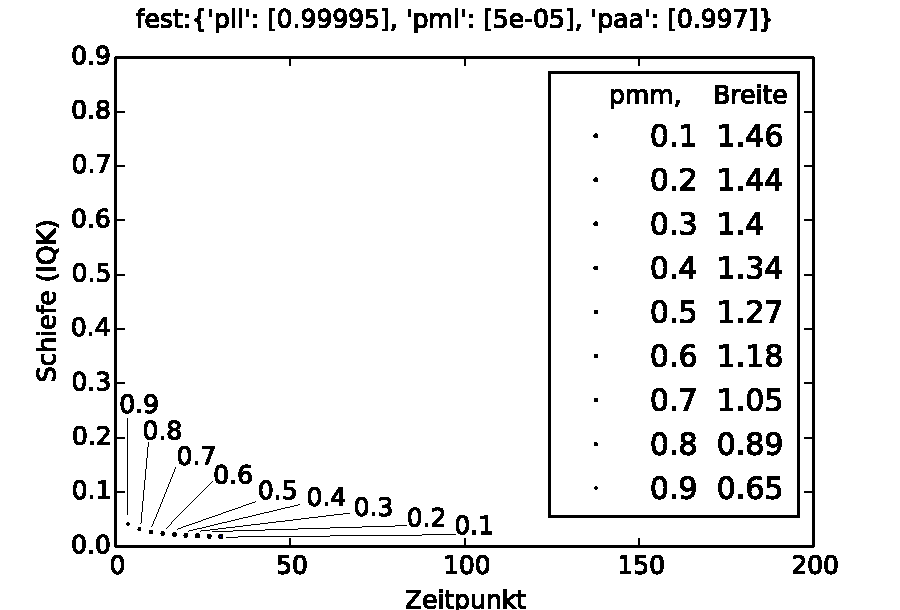
\includegraphics[width=\textwidth]{bilder/3fest_p_000005_0997_099995.pdf}
\caption{$p_{mm}$ und $p_{ml}$ groß}
\end{subfigure}
\begin{subfigure}[t]{0.5\textwidth}
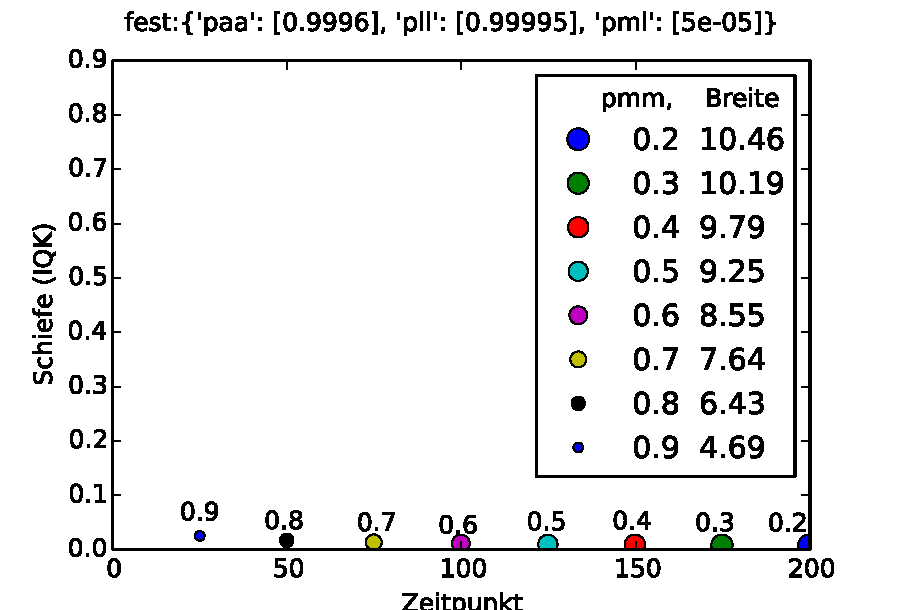
\includegraphics[width=\textwidth]{bilder/3fest_p_000005_09996_099995.pdf}
\caption{$p_{mm}$ groß und $p_{ml}$ klein}
\end{subfigure}
\caption{Der Einfluss von $p_{mm}$ auf die Breite abhängig von $p_{mm}$}
\label{einfluss_pmm_1}
\end{figure}

Wie in Abbildung \ref{einfluss_pmm_1} zu sehen, ist der Einfluss von $p_{mm}$ auf den Zeitpunkt von $p_{aa}$ abhängig: Je größer $p_{aa}$ ist, desto stärker wird der Zeitpunkt von $p_{mm}$ beeinflusst. Wenn $p_{mm}$ und $p_{aa}$ klein sind, entstehen nur Peaks zu Beginn des Spektrums, unabhängig von $p_{ml}$ oder pll.
Der Einfluss von $p_{mm}$ auf die Breite ist gering, bei größerem PAA steigt dieser Einfluss etwas, wie ebenfalls in Abbildung \ref{einfluss_pmm_1} zu erkennen ist. Dieser Einfluss hängt damit zusammen, dass sich in diesem Fall auch der Maximalzeitpunkt nach hinten verschiebt und spätere Peaks generell breiter sind, als frühe Peaks.
%, was aber wahrscheinlich auch mit dem in diesem Fall ansteigenden Zeitpunkt zu tun hat (Peaks haben dem maxzeitpunkt auf dem gesamten Spektrum und werden mit zunehmender Zeit auch breiter)

% \begin{figure}[H]
% \begin{subfigure}[t]{0.5\textwidth}
% \includegraphics[width=\textwidth]{bilder/}
% \caption{$p_{aa}$ groß und $p_{ml}$ groß}
% \end{subfigure}
% \begin{subfigure}[t]{0.5\textwidth}
% \includegraphics[width=\textwidth]{bilder/}
% \caption{$p_{aa}$ groß und $p_{ml}$ klein}
% \end{subfigure}
% \vspace*{7mm}
% \begin{subfigure}[b]{0.5\textwidth}
% \includegraphics[width=\textwidth]{bilder/}
% \caption{$p_{aa}$ klein und $p_{ml}$ groß}
% \end{subfigure}
% \begin{subfigure}[b]{0.5\textwidth}
% \includegraphics[width=\textwidth]{bilder/}
% \caption{$p_{aa}$ klein und $p_{ml}$ klein}
% \end{subfigure}
% \caption{Der Einfluss von $p_{mm}$ auf die Schiefe abhängig von $p_{aa}$, $p_{ml}$ und $p_{ll}$}
% \label{einfluss_pmm_2}
% \end{figure}


TODO: Noch mal den kleinen Bereich untersuchen, wo die Schiefe negativ beeinflusst wird. Das ist ein Bereich, in dem die Peaks zwar sehr früh, aber dafür fast zu breit sind. Vielleicht hängt das damit zusammen? siehe: $p_{mm}$0.001 0.998 0.99999
Ansonsten steigt die Schiefe mit steigendem pmm. Dieser Einfluss hängt noch von $p_{aa}$ab, bei kleinem $p_{aa}$hat $p_{mm}$einen größeren Einfluss auf die Schiefe. Hängt aber auch von pml/pll ab! 
Einfluss am nur vorhanden bei mittlerem $p_{ml}$ (0,0001, 0,0005). Ist $p_{ml}$ zu klein, hat die Lösung fast keinen Einfluss, ist $p_{ml}$zu groß, werden die Peaks wieder nur breit, aber nicht so schief. Gleiches gilt für $p_{ll}$ (pmm beeinflusst Schiefe bei $p_{ll}$ von 0,99995-0,99999).
Wahrscheinlich, weil dadurch, dass $p_{aa}$ klein ist, der Einfluss von $p_{ml}$ und $p_{ll}$ größer wird. $p_{ml}$ und $p_{ll}$ verursachen ja gemeinsam das Tailing, dieser Tailingeffekt kann sich aber nur bei großem $p_{mm}$ durchsetzen, da die Teilchen, die nicht in den gelösten Zustand kommen, sich recht schnell fortbewegen (daher auch besonders bei kleinem $p_{aa}$ zu beobachten) und dadurch nur wenige Teilchen langsamer sind und dadurch den Tail verursachen. Ist kleiner, lösen sich die Teilchen häufiger und statt der schiefen entstehen breite Peaks
Ist $p_{aa}$ zu klein und $p_{ll}$ zu groß entstehen peaks, die zwar einen extrem großen iqk haben. Allerdings ist der Tail so flach, dass er in einem Gesamtchomatogramm wohl eher im Rauschen untergehen würde.


\begin{figure}
\begin{subfigure}[t]{0.5\textwidth}
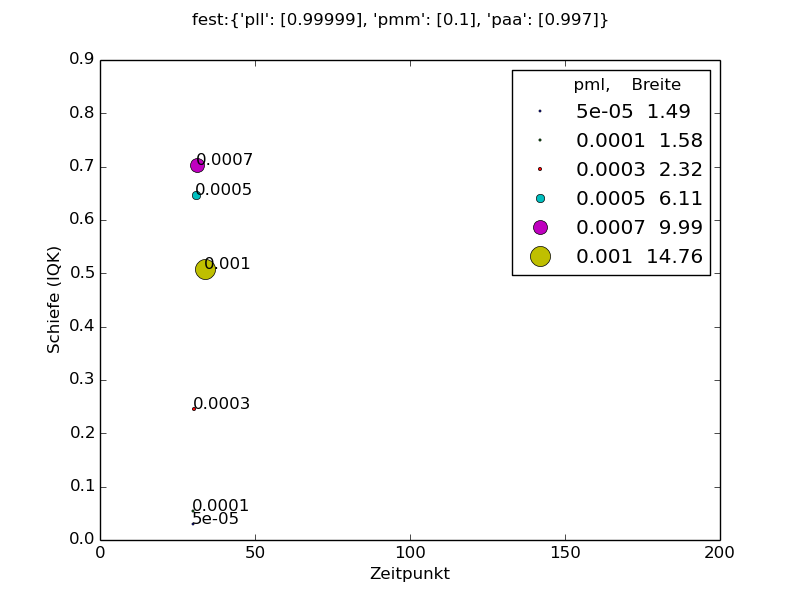
\includegraphics[width=\textwidth]{bilder/pml/pml_01_p_0997_099999}
\caption{$p_{ll}$ sehr groß}
\end{subfigure}
\begin{subfigure}[t]{0.5\textwidth}
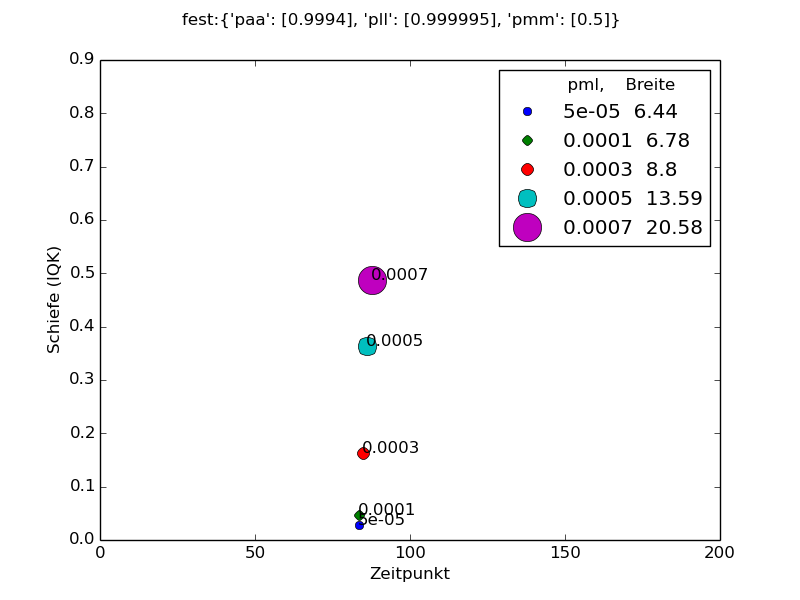
\includegraphics[width=\textwidth]{bilder/pml/pml_05_p_09994_0999995}
\caption{$p_{ll}$ groß}
\end{subfigure}
\vspace*{7mm}
\begin{subfigure}[b]{0.5\textwidth}
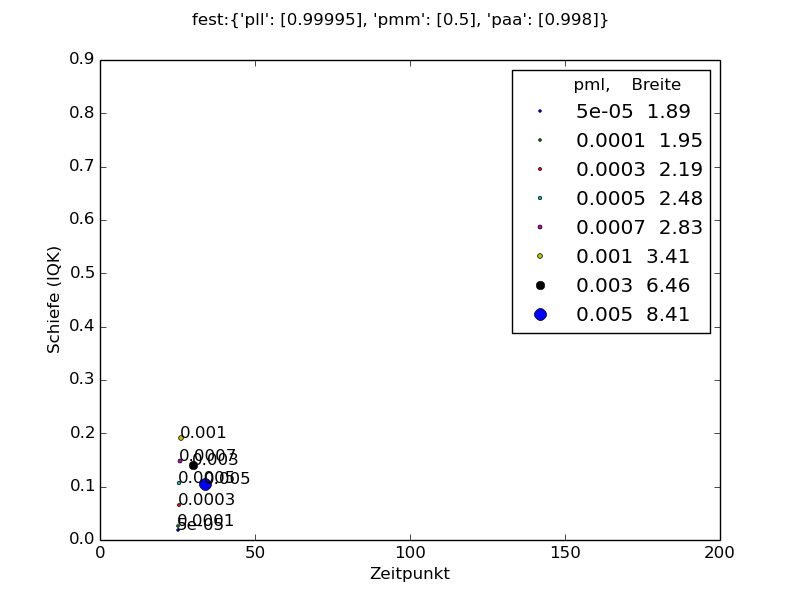
\includegraphics[width=\textwidth]{bilder/pml/pml_05_p_0998_099995}
\caption{$p_{ll}$ klein}
\end{subfigure}
\begin{subfigure}[b]{0.5\textwidth}
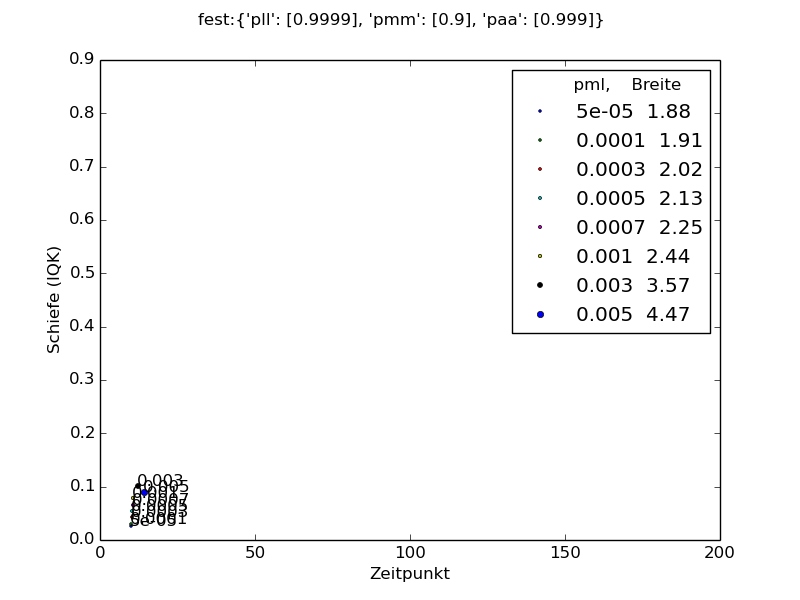
\includegraphics[width=\textwidth]{bilder/pml/pml_09_p_0999_09999}
\caption{$p_{ll}$ sehr klein}
\end{subfigure}
\caption{Der Einfluss von $p_{ml}$ auf die Schiefe und Breite abhängig von $p_{ll}$}
\label{einfluss_pml_1}
\end{figure}

Der Einfluss von $p_{ml}$ auf die Peakdaten ist in Abbildung \ref{einfluss_pml_1} gezeigt. Der Zeitpunkt ist nur minimal von pml abhängig. Die Punkte liegen fast auf einer Geraden oder nur leicht schrägen Linie nach oben. Allenfalls sehr große Werte für pml sorgen für einen deutlich erkennbaren höheren Zeitpunkt, dann aber auch für deutlich mehr Breite und weniger Schiefe.
Auf die Schiefe ist der Einfluss von pml sehr groß, wenn auch $p_{ll}$ groß ist. Gleiches gilt für die Breite, auch diese wird nur deutlich von pml beeinflusst, wenn auch pll groß ist. 

\begin{figure}
\begin{subfigure}[t]{0.5\textwidth}
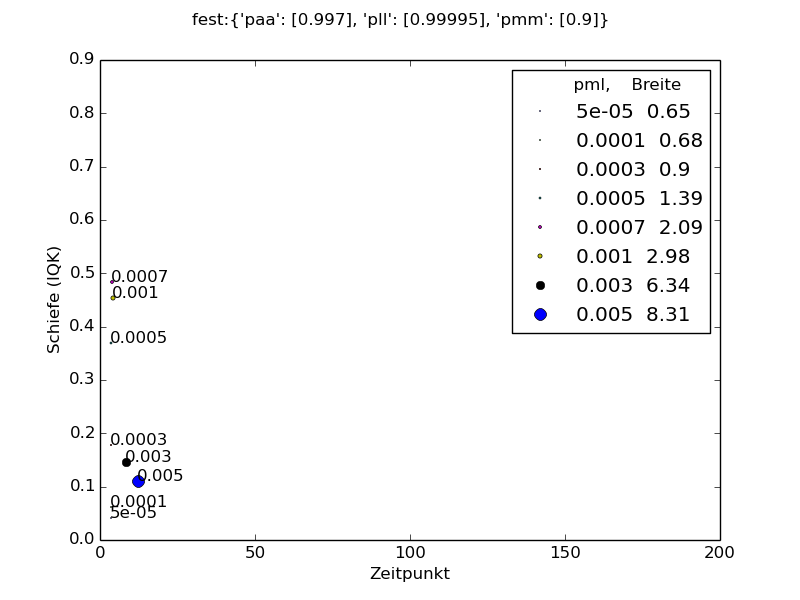
\includegraphics[width=\textwidth]{bilder/pml/pml_09_p_0997_099995}
\caption{$p_{mm}$ groß, paa klein}
\end{subfigure}
\begin{subfigure}[t]{0.5\textwidth}
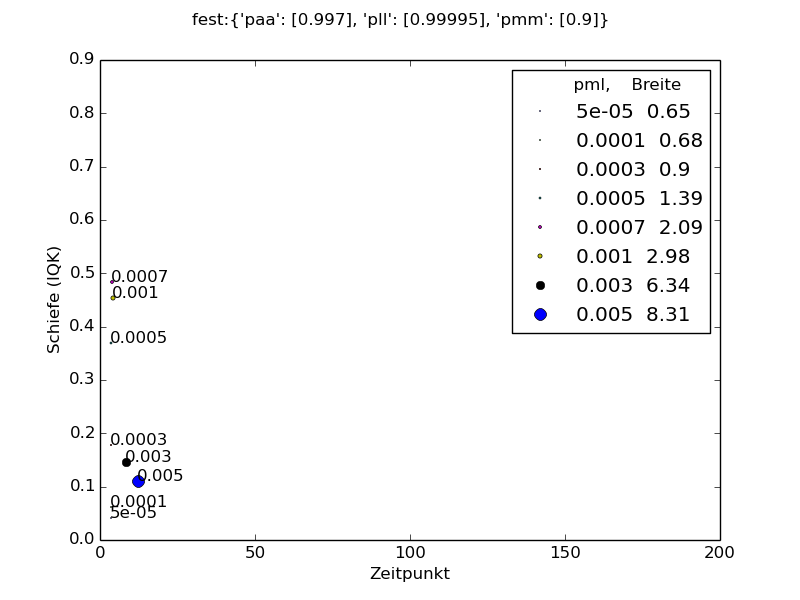
\includegraphics[width=\textwidth]{bilder/pml/pml_09_p_0997_099995}
\caption{$p_{mm}$ groß, paa groß}
\end{subfigure}
\vspace*{7mm}
\begin{subfigure}[b]{0.5\textwidth}
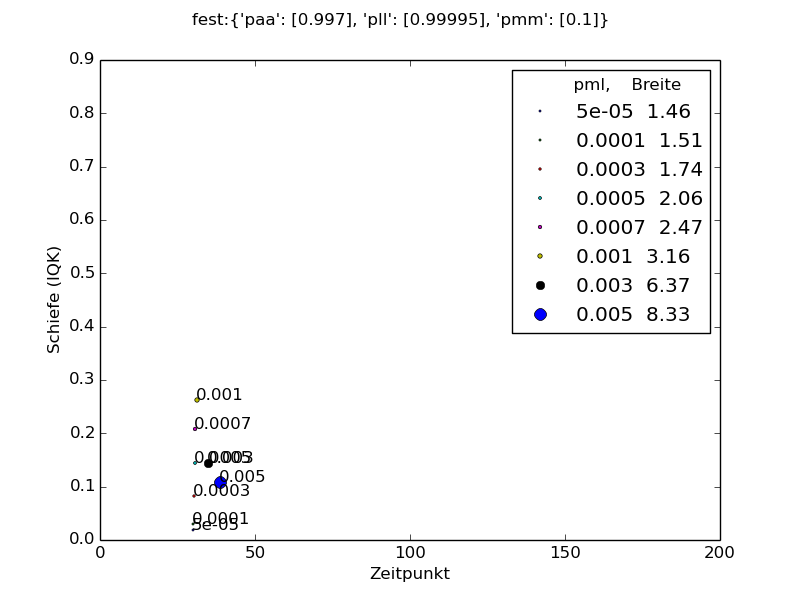
\includegraphics[width=\textwidth]{bilder/pml/pml_01_p_0997_099995}
\caption{$p_{mm}$ klein, paa klein}
\end{subfigure}
\begin{subfigure}[b]{0.5\textwidth}
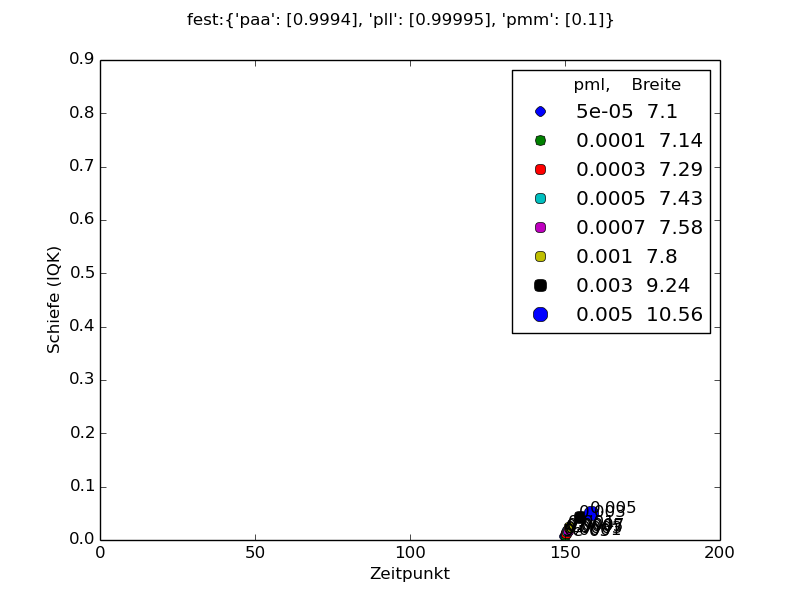
\includegraphics[width=\textwidth]{bilder/pml/pml_01_p_09994_099995}
\caption{$p_{mm}$ klein, paa groß}
\end{subfigure}
\caption{Der Einfluss von $p_{ml}$ auf die Schiefe und Breite abhängig von $p_{mm}$ und paa}
\label{einfluss_pml_2}
\end{figure}

Wie in Abbildung \ref{einfluss_pml_2} gezeigt, spielen auch pmm und paa für den Einfluss von pml nur eine  Rolle. Ist paa klein, wird der Einfluss von pml auf Schiefe und Breite größer, ist pmm klein, wird der Einfluss auch kleiner.


%, wie ebenfalls in Abbildung \ref{einfluss_pml} zu erkennen ist.


Evtl eher verschiedene Werte für pll als nur zwei zeigen, da erkennt man evtl mehr



\begin{figure}[H]
\begin{subfigure}[t]{0.5\textwidth}
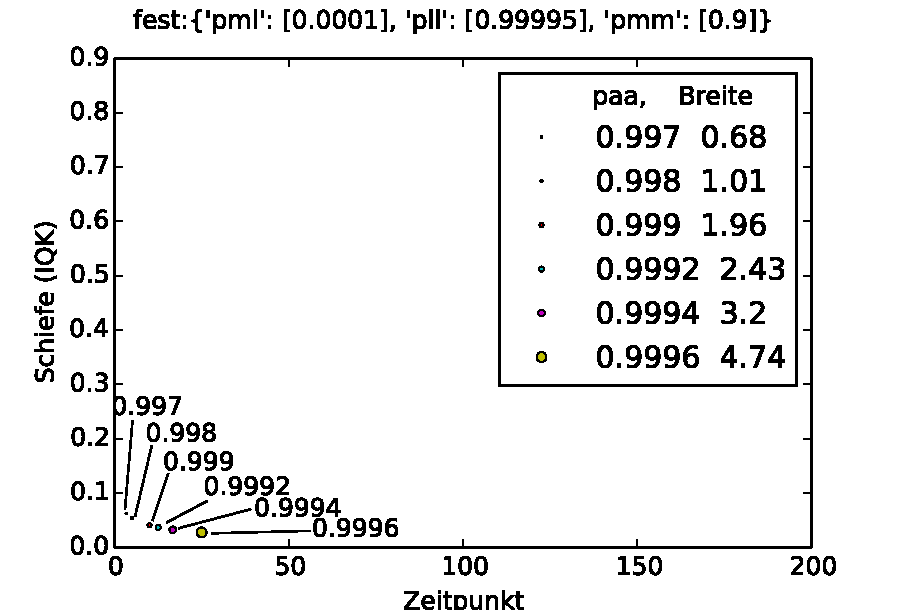
\includegraphics[width=\textwidth]{bilder/3fest_09_00001_p_099995.pdf}
\caption{$p_{mm}$ und $p_{ml}$ groß}
\end{subfigure}
\begin{subfigure}[t]{0.5\textwidth}
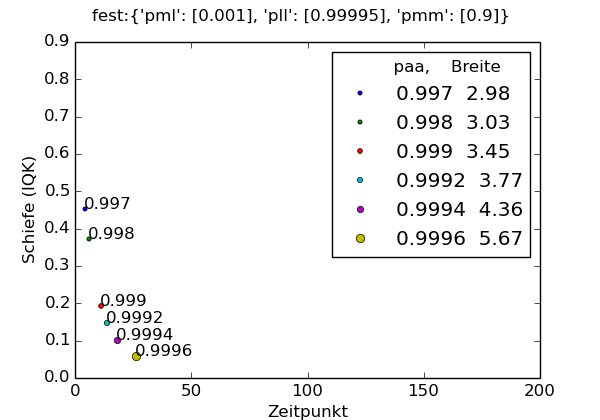
\includegraphics[width=\textwidth]{bilder/3fest_09_0001_p_099995}
\caption{$p_{mm}$ groß und $p_{ml}$ klein}
\end{subfigure}
\vspace*{7mm}
\begin{subfigure}[b]{0.5\textwidth}
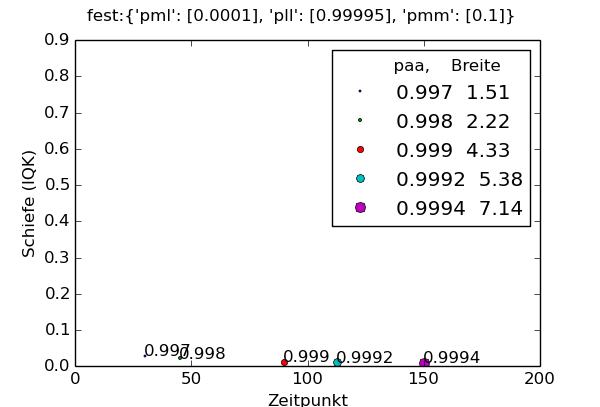
\includegraphics[width=\textwidth]{bilder/3fest_01_00001_p_099995}
\caption{$p_{mm}$ klein und $p_{ml}$ groß}
\end{subfigure}
\begin{subfigure}[b]{0.5\textwidth}
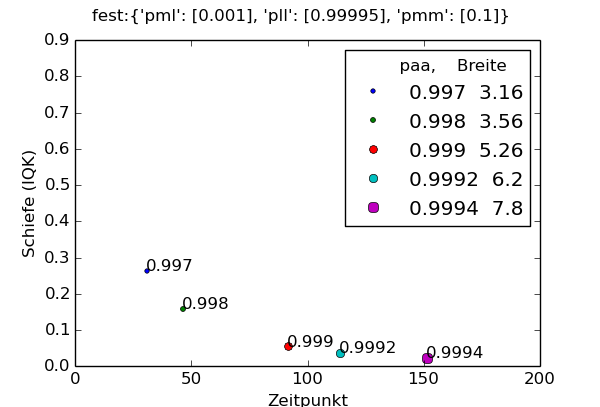
\includegraphics[width=\textwidth]{bilder/3fest_01_0001_p_099995}
\caption{$p_{mm}$ und $p_{ml}$ klein}
\end{subfigure}
\caption{Der Einfluss von $p_{aa}$ auf die Peaks abhängig von $p_{mm}$ und $p_{ml}$}
\label{einfluss_paa}
\end{figure}

In Abbildung \ref{einfluss_paa} ist beispielhaft der Einfluss von Parameter $p_{aa}$ auf die Peaks gezeigt. Der Einfluss von $p_{aa}$ auf den Zeitpunkt wird mit steigendem $p_{mm}$ immer kleiner und reicht dadurch von minimalem Einfluss und recht frühen Peaks bei jeder Wahl von $p_{aa}$ bis zu sehr großem Einfluss und Peaks, die je nach $p_{aa}$ über das ganze Spektrum verteilt sind. Damit hat $p_{aa}$ einen ähnlichen Einfluss wie pmm. $p_{aa}$ hat nur dann einen relevanten Einfluss auf die Schiefe, wenn $p_{ml}$ groß ist. Der Einfluss auf die Breite ist mäßig und wird größer, wenn $p_{ml}$ und $p_{ll}$ klein sind.

Der Einfluss von $p_{ll}$ auf den Zeitpunkt ist minimal (Punkte liegen mehr oder weniger alle auf einer fast geraden nach oben)

\section{Laufzeiten}

% diskussion.tex
\chapter{Diskussion}
\label{chapter:dis}
\todo{Kapitel Diskussion schreiben}

\section{Ergebnisse}
Es wurde ein Zusammenhang zwischen den Simulationsparametern und Peakdaten gefunden.


\section{Ausblick}

% Bessere bzw. genauere Aufarbeitung der Referenzdaten: Methoden, die ztatsächlichen Peaks gut zu isolieren (\todo{kann man hier auf bestehende Arbeiten zur peakfindung verweisen?}) evtl. feinere Daten durch schätzen weiterer zwischenmessungen, um glattere Daten zu erhalten? Verfahren umd zu erkennen, ob Peaks gut sind für den Vergleich
Das ganze mit existierenden Daten vergleichen, um zu gucken, ob schmalere Peaks notwendig sind und alle realen Peakdatenkombinationen erreicht werden können, dann eventuell noch mal das Modell anpassen:
Tailform richtig?

Je nachdem, ob die bisherigen Ergebnisse ausreichen, um eine größere Anzahl im Experiment gefundener Peaks zu simulieren, können die am Ende von Kapitel \ref{chapter:mod} erwähnten Ideen für weitere Modellveränderungen ausprobiert werden. Sowohl die Berücksichtigung des Gleichgewichts der Phasen als auch eine maximale Kapazität für die Adsorption können für weiteres Tailing sorgen. Außerdem ist es auch gut vorstellbar, dass so schmalere Peaks zum gleichen Zeitpunkt entstehen, da sich für einige Teilchen die Wahrscheinlichkeit, mobil zu bleiben erhöht und ein Teilchenpulk enger beieinander bleibt.

Aufgreifen der nicht umgesetzten Modellerweiterungen: Berücksichtigung des Gleichgewichts der Phasen und beschränkte Anzahl freier Plätze bei der Adsorption.

Eine weitere Möglichkeit, das Modell zu verändern, besteht darin, das Gleichgewicht, welches sich zwischen den beiden Phasen aufbaut, zu berücksichtigen. Damit müssten die Wahrscheinlichkeiten, den Zustand zu wechseln, nicht mehr fest vorgegeben sein, sondern sich dynamisch während der Simulation aus der aktuellen Verteilung der Teilchen an einem bestimmten Ort auf die Zustände berechnen.

Außerdem existieren Idee, noch eine Sättigung der freien Plätze zur Adsorption einzubauen

Das ganze auch für spätere Zeitpunkte überprüfen (echte Messlänge, dauert nur halt lange mit der Sim, evtl dafür die eventsim nutzbar?)

Falls Formel für entsprecung nicht gefunden: Das Sekantenverfahren erwähnen?
Verfahren entwickeln, um gewünschten Peak zu simulieren. Bisher funktioniert das händisch unter Anwendung der Erkenntnisse, wie sich die Parameter auf die Peaks auswirken. Wenn also ein Peak mit bestimmten Eigenschaften gewünscht ist, wird bisher die grobe Umgebung abgesucht. Die Parameter der dort gefundenen Peaks werden in die passende Richtung abgewandelt (zb. er ist etwas zu früh, dann wird pmm verringert oder zu schmal, dann wird pll erhöht). Anschließend wird überprüft, wo der neue Peak liegt und evtl noch mal die Parameter angepasst. 
Um das zu ersparen müsste entweder der komplette Parameterraum noch besser abgedeckt werden (was uU sehr viel Laufzeit und Speicherplatz kostet) oder die Vorgehensweise automatisiert werden.

Umsetzung von Modellen mit mehr Zuständen: Simulation als event nicht schwer (und von den Laufzeiten her wohl auch ganz gut) die by-step müsste aber angepasst werden (Schleifen) da sonst wohl zu aufwändig und zu langsam. gleiches gilt für paa, da wäre auch eine neue umsetzung nötig

Doch noch mal Halbwertsbreite bzw 10\% Breite und Breite links und rechts des Maximums als Maße für Breite und Schiefe testen, da in einigen Fällen die berechneten Werte den vom menschlichen Betrachter gewonnenen Eindruck widersprechen.

\cleardoublepage
% Anhang
%\appendix
%% anhang.tex
\chapter{Weitere Informationen}


%Abbildungsverzeichnis
\listoffigures
\addcontentsline{toc}{chapter}{Abbildungsverzeichnis}
\cleardoublepage

% Algorithmenverzeichnis
%\listofalgorithms
%\addcontentsline{toc}{chapter}{Algorithmenverzeichnis}
%\cleardoublepage

% Literaturverzeichnis
%\bibliographystyle{gerplain}
\bibliographystyle{plainnat}
\bibliography{literatur/diplom}
\addcontentsline{toc}{chapter}{\bibname}

% Erklaerung
%\thispagestyle{myheadings}
%\markboth{}{ERKLÄRUNG}
%\addcontentsline{toc}{chapter}{Erklärung}
%% erklaerung.tex
\cleardoublepage
\normalsize
Hiermit versichere ich, dass ich die vorliegende Arbeit selbstständig verfasst habe und keine anderen als die angegebenen Quellen und Hilfsmittel verwendet sowie Zitate kenntlich gemacht habe.\\\\
Dortmund, den \today \\\\\\\\
Elisabeth Böhmer
%\cleardoublepage

\end{document}
% EOF
